%\section{Introduction}
As shown previously in multiple applications in the literature, dynamic reconstruction can improve activity and parametric image estimates by making use of dynamic models directly in the reconstruction process, resulting in more accurate modelling of the noise from the raw PET data~\cite{Reader2014}. 

In this chapter, we shortly describe the implementation of a dynamic reconstruction framework and dynamic reconstruction functionalities in CASToR. A fraction of this PhD project was focused on the development and validation of these functionalities that were necessary to achieve the project aims. The developments were conducted in collaboration with other CASToR developers, mainly with Dr Thibaut Merlin, Dr Simon Stute and Dr Marina Filipović.
In addition, dynamic functionalities were implemented within a generic framework that allows for future expansion and contributions by developers of CASToR, to include more dynamic models and enable more complex and higher dimensional modelling (eg. dynamic and respiratory "5D" modelling , etc.).

In the remaining of this chapter, we present work conducted with simulated and real data on the use and respective benefits of various dynamic reconstruction strategies for DWB parametric imaging. This study has been submitted to the journal of \textbf{Physics in Medicine \& Biology} for review in May 2021. 

\section*{Introduction}
Positron Emission Tomography (PET) imaging is well known and established in clinical applications and pathways, with an important role towards the delivery of precision medicine~\cite{Subramaniam2017}. The established clinical practices rely on static imaging after a certain uptake period and semi-quantitative measures, such as the standardised uptake value (SUV). But these measures are vulnerable to many unknown factors that can vary between PET examinations, such as body composition, retention clearance, inconsistencies in uptake time and imaging practices~\cite{Boellaard2011}. On the other hand dynamic PET imaging can be used to fully characterise underlying tracer kinetics and provide fully quantitative measures, that could overcome many limitations of current static imaging practices and enable use of PET for new applications in clinical practice~\cite{Lammertsma2017,Dimitrakopoulou2021,Meikle2021}. \\
Current clinical scanners are limited in coverage by their axial field of view (A-FOV), with values ranging from 15 to 26 cm \cite{Vandenberghe2020}. This is sufficient for single organ dynamic studies but cannot directly provide synchronous whole-body coverage, which is essential for some clinical applications such as tumour staging in oncology. 
In practice for static imaging whole-body coverage is achieved using multiple bed positions at different axial locations to provide the desired axial coverage~\cite{Schubert1996}, or alternatively via continuous axial bed motion (CBM) during the acquisition~\cite{Panin2014}. 
Recently scanners with increased A-FOV have been developed~\cite{Karp2020,Siegel2020},
even with nearly 2 meters long A-FOV which provides total-body coverage~\cite{Cherry2018}. 
But these scanners are still not widely adopted in the clinic. 
Using similar methods as in static whole-body imaging, dynamic whole body (DWB) protocols have been developed using multiple bed positions and repeated whole-body passes~\cite {Karakatsanis2011,Karakatsanis2013,Rahmim2019}. These types of acquisition protocols have also been incorporated into clinical products~\cite{Hu2020}, and it has been shown that their use in clinical practice is feasible~\cite{Fahrni2019,Dias2020}. \\
The immediate effect of transition from single bed dynamic studies to multi-bed dynamic studies is the introduction of temporal gaps in the acquired data of any given bed position. 
These are introduced at each bed position by the time spent on imaging other bed positions and by scanner system delays due to the time required to move the bed to the next position and prepare for the next acquisition.
These gaps cause a significant reduction in the sensitivity of the acquisition, with fewer total counts collected for each axial location when compared to single bed dynamic acquisitions. Furthermore, estimation of fast temporal changes in tracer uptake are compromised as the early time points of the acquisition are not fully sampled for all beds. Finally the established clinical protocols that make use of image derived input function (IDIF) to ease integration in clinical practice further sacrifice imaging time in the study’s early phase, which is spent in acquiring fast frames over a single bed location centred over the heart and the aorta~\cite{Hu2020}. \\
The generation of parametric images from dynamic data requires fitting of the dynamic model of interest on time activity curves (TAC) for every voxel in the image. 
Due to the poor statics and high noise associated with TAC measurements at the voxel level, in particular for DWB acquisitions, parametric image estimates can be heavily corrupted by noise and potentially biased. 
The use of direct dynamic reconstruction has been proposed to improve on this task by making use of dynamic models directly in the reconstruction. These techniques allow for more accurate modelling of the noise from the raw PET data in the generation process of parametric images and can improve parametric image noise and reduce bias~\cite{Reader2014}. For DWB acquisitions specifically, it has been shown using simulated and real data that direct dynamic reconstruction provides reduced noise, bias and improved parametric image contrast when compared to post-reconstruction parametric imaging~\cite{Karakatsanis2016a}.\\
In this work, we evaluate the performance of dynamic reconstruction algorithms for DWB fluorodeoxyglucose ([$^{18}$F]FDG) PET imaging for various dynamic reconstruction methods and for different DWB acquisition protocols. The evaluation is based on simulations of single bed and multi-bed dynamic studies and results are illustrated in a real dynamic FDG PET study.


In detail we evaluate for WB Patlak $K_i$ parametric imaging 
(1) the benefits of using direct Patlak dynamic reconstruction in DWB protocols against single bed dynamic protocols and indirect parametric imaging from regular 3D reconstruction, 
(2) the use of the Spectral analysis dynamic model~\cite{Cunningham1993} in dynamic reconstruction for indirect parametric imaging,
(3) the use of two different optimization algorithms for dynamic reconstruction
and finally (4) the impact of different DWB acquisition strategies.

\section*{Methods}

\subsection*{Simulated acquisition protocols}
A single bed (SB) dynamic protocol (continuous in time with no temporal gaps) and three DWB acquisition protocols of five bed positions (with temporal gaps) were simulated for this study, using the geometry characteristics of the GE Signa PET/MR scanner~\cite{Grant2016}. With the provided 25 cm A-FOV per bed and a bed overlap of 3.34 cm, axial coverage of 110.3 cm can be achieved with five bed positions. The relatively small overlap (approximately half compared to routine clinical protocols) was selected to reduce the number of beds and subsequently the acquisition temporal gaps.
%All three DWB protocols mimic the timing characteristics of the Signa PET/MR but differ in acquisition strategy.
A total study duration of 60 minutes was used in the design of all protocols, including an initial single bed dynamic phase of 3 minutes centred over the aorta to mimic requirements for IDIF estimation.

\begin{itemize}
\item The first DWB protocol (DWB-1) considers a step and shoot (S\&S) acquisition using the timing characteristics of the Signa PET/MR, with a delay of 6 seconds between adjacent bed positions and 36 seconds between whole-body sweeps, resulting to 8 whole-body sweeps in the duration of the study. \\

\item The second DWB protocol (DWB-2) differs from DWB-1 by use of system delays that mimic a continuous bed motion (CBM) acquisition of the same length, with no delays between adjacent bed positions and 12 seconds delay between whole-body sweeps to account for bed speed and acquisition overscan (used to obtain reasonable axial sensitivity at the edges of the acquisition~\cite{Panin2014}). This protocol results to 9 whole-body sweeps. The actual simulation for DWB-2 did not make use of continuous bed motion in the simulation process but made use of the accurate timings that reflect reduction of delays and framing achieved with CBM on the same system geometry. This is conceptually equivalent to CBM sinogram data (sometimes refereed as "chunks"~\cite{Hu2014}) with uniform framing over the FOV instead of slice-dependent timings as in actual CBM sinograms. \\

\item The third DWB protocol (DWB-3) replicates the timing properties of DWB-2 for CBM acquisition but utilises a bi-directional acquisition that reduces delays between sweeps to the time spent for the over-scan. This acquisition motion provides more sweeps in the same study duration but results in non-uniform sampling. This protocol results to 10 whole-body sweeps.
% for the 2nd and 4th bed positions. \\
\end{itemize}
\noindent 
Our study focuses on the second axial bed location for the DWB simulations, centred over the upper chest as seen in figure~\ref{fig:DWBprotocols}.
The PET data simulations were conducted solely for this bed position using the framing of the protocols described above. The exact framing information are available in appendix~\ref{chap:AppendixB}.%  as shown in table~\ref{table:FrameTimings}.

\textcolor{blue}{
A fourth DWB protocol (DWB-4) was simulated in addition to the above protocols, for evaluating parameters estimation that depends on early dynamic information. For this protocol the timing of the DWB-1 was considered, with the addition of the early dynamic single bed information that was split into nine frames of 20 seconds each.}


\begin{figure} [ht!]
\centering
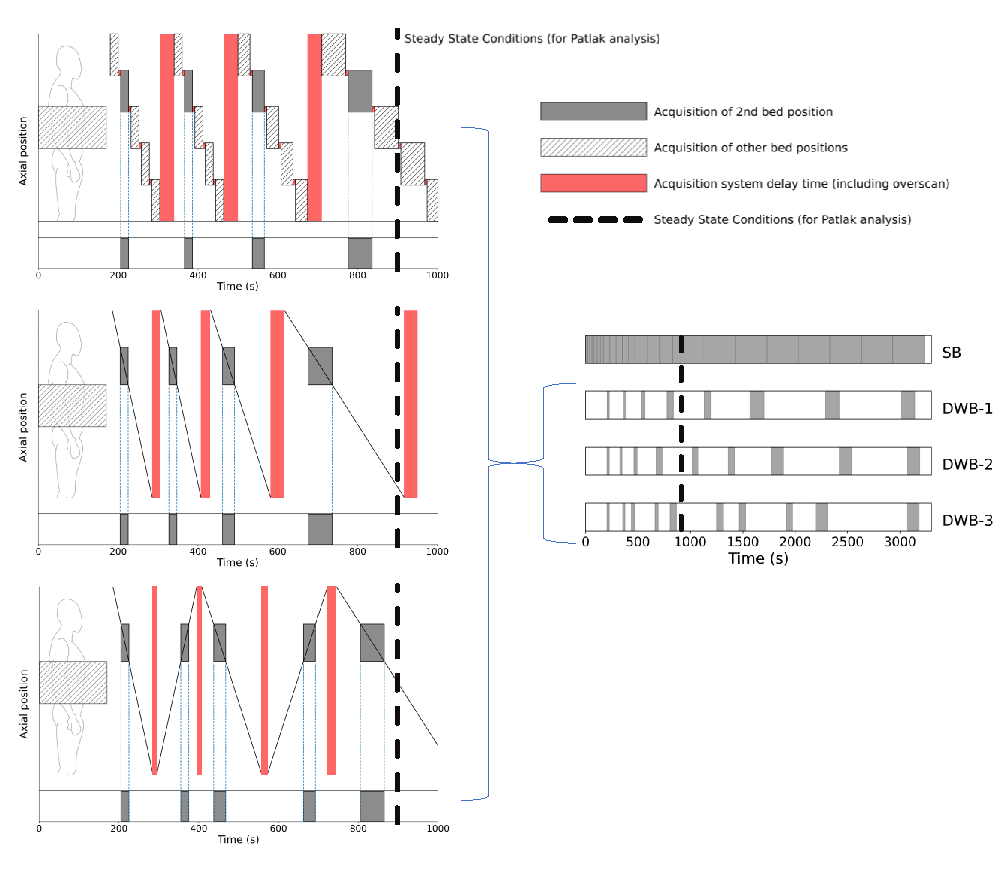
\includegraphics[scale=1.03,angle=0]{3_Results/3_2_Dynamic_Reconstruction_SimulationStudy/figures/protocols.pdf}
\caption{Dynamic whole-body acquisition protocols considered for simulation.} 
%TODO: Add over-scan in the CBM D-WB protocols. 
\label{fig:DWBprotocols}
\end{figure}

\begin{figure} [ht!]
\centering
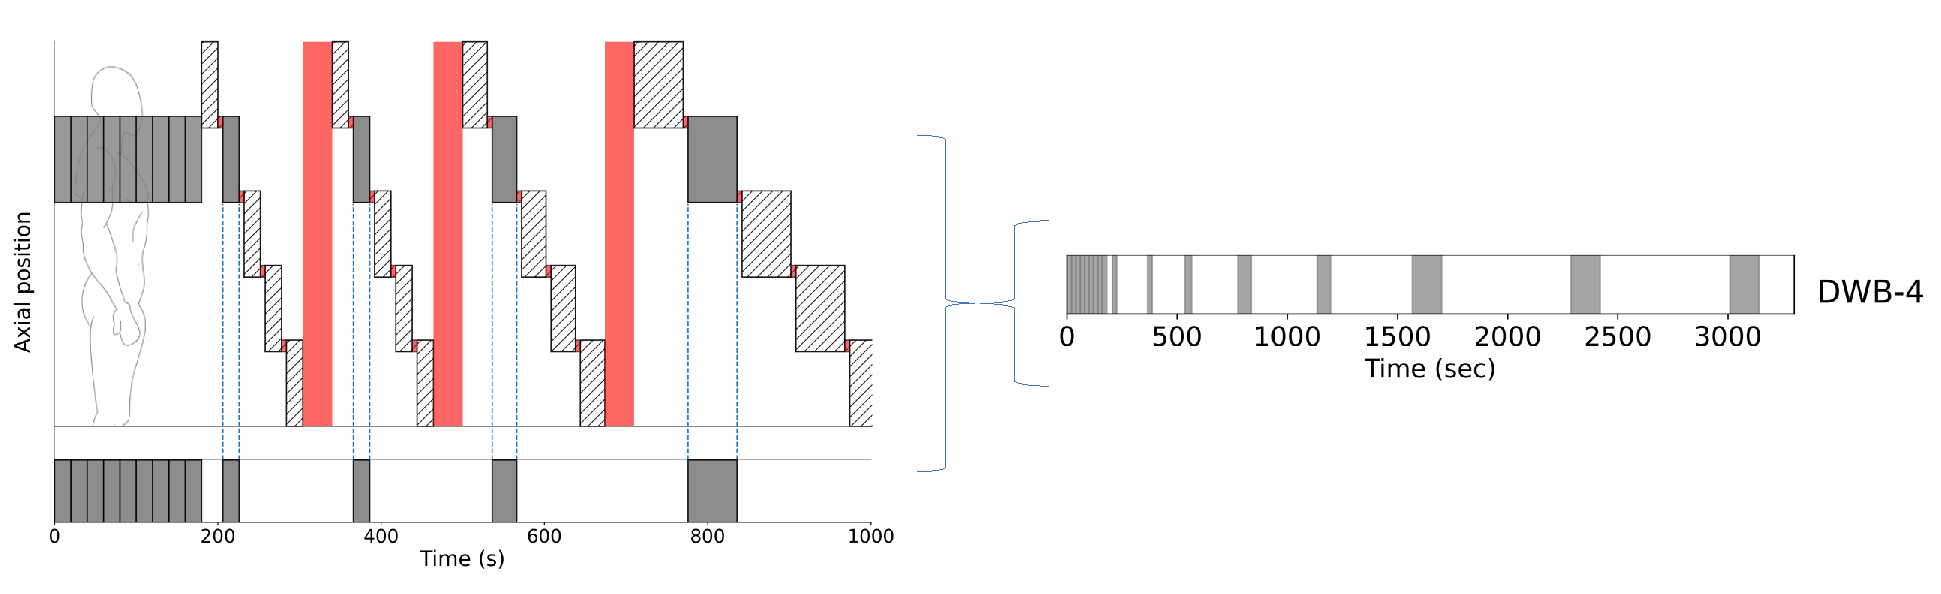
\includegraphics[scale=0.52,angle=0]{3_Results/3_2_Dynamic_Reconstruction_SimulationStudy/figures/AdditionalProtocolDWB4.pdf}
\caption{Fourth dynamic whole-body acquisition protocol considered for simulation, which includes the initial single bed dynamic phase.} 
%TODO: Add over-scan in the CBM D-WB protocols. 
\label{fig:DWB4_Protocol}
\end{figure}

\subsection*{Digital phantom \& analytical simulation}
The Zubal brain phantom~\cite{Zubal1994} was chosen for the simulations of PET [$^{18}$F]FDG data, even though its anatomy doesn't correspond to the anatomy that would be found in the axial location of the simulated bed position. The choice of the phantom was made to incorporate higher complexity structures than those offered from common lung/chest phantoms. Furthermore the use of the brain phantom, centred in the FOV, aided in avoiding analysis of areas falling in the overlapping regions, whose behaviour under DWB acquisition and reconstruction is yet another subject for investigation. The Zubal brain phantom was segmented into 19 unique regions and a non-reversible two tissue compartment model was assigned uniformly to each region to simulate realistic FDG kinetics, with $K_1$, $k_2$, $k_3$ and $V_b$ values drawn from the literature and a real measured input function. A selection of the simulated kinetic parameters is provided in appendix~\ref{chap:AppendixB}.
An analytical simulator was used to generate raw PET sinogram data~\cite{Stute2015}. The simulations included attenuation and detector resolution effects, scattered and random coincidences, while Poisson noise was added to the sinogram data. % to \textbf{match noise levels from typical FDG-PET examinations performed on the Signa PET-MR}.
The simulation did not include time of flight (TOF) information in the data. Fifty different noise realisations were simulated for each DWB protocol. For the SB protocol the number of noise realisation was reduced to twenty as simulation and reconstruction times of the SB datasets were substantially higher.

\subsection*{Reconstruction and kinetic modelling}
Both 3D and dynamic iterative reconstructions were used. All reconstructions were run within an OSEM framework, for 40 iterations and 28 subsets, using the open source fully quantitative reconstruction platform CASToR~\cite{Merlin2018}. 
All reconstructions were performed with a voxel size of $2.2~\mathrm{mm}\times2.2~\mathrm{mm}\times2.8~\mathrm{mm}$ and included resolution modeling as well as corrections for attenuation and for random and scattered coincidences (generated from the simulation).
Dynamic reconstructions are made by combining dynamic models that describe the tracer kinetics with the tomographic reconstruction process. When the dynamic model of interest is used this technique results in direct reconstruction of parametric images of interest and allows for accurate modeling of the raw data noise in the estimation process~\cite{Carson1985,Matthews1995,Kamasak2003,Wang2008}. Use of generic dynamic models can also be made for dynamic reconstruction, where dynamic models impose temporal regularisation in the frame activity estimation process. Post-reconstruction (indirect) estimation of parametric images can then be made and indirectly benefit from the use of dynamic reconstruction~\cite{Reader2014,Novosad2016b}.
Linear dynamic models can be directly implemented within the system matrix~\cite{Matthews1995,Wang2008,Reader2014} but result in algorithms with substantially slower overall convergence properties.
Instead a nested optimization framework~\cite{Wang2010,Matthews2010} can be used, which decouples the dynamic model fitting process on image space data from the tomographic update process over the raw PET data. This allows for multiple nested sub-iterations of dynamic model fitting to be run within each tomographic iteration of the reconstruction process, resulting in convergence acceleration and reasonable computing time requirements.
The separation of the two processes allows for various optimization algorithms to be implemented in the nested dynamic model fitting process~\cite{Matthews2010}. One particular method of interest is the Non-Negative Least Squares (NNLS) algorithm~\cite{Lawson1995}, that enforces non-negativity and is commonly used in post-reconstruction kinetic modeling. The NNLS algorithm is self-terminating and for dynamic reconstruction it has been shown that a single execution of nested NNLS results to parametric images with similar Root Mean Square Error (RMSE) to that of 15 iterations of nested MLEM~\cite{Matthews2010}. Therefore use of nested NNLS optimization has the potential for reduced overall reconstruction times.
In this work we made use of both nested MLEM and NNLS optimizations to compare their performance and reconstruction time requirements for their implementation within CASToR. 
The nested MLEM optimization was used with 20 sub-iterations of the dynamic model fitting process after each subset of the OSEM tomographic update process, which has been found to be the optimal number of sub-iterations in a previous similar study~\cite{Karakatsanis2016a}.  
Hereafter we will refer to nested dynamic reconstruction simply as \mbox{\textit{4D reconstruction}}. 

In this work we evaluated two different linear dynamic models for 4D reconstructions, the Patlak model and the Spectral analysis model.

\begin{itemize}
\item 4D Patlak: 

The Patlak model describes the activity in tissue ${C_{T}}(t)$ as
\begin{equation} \label{Patlak}
{C_{T}}(t) = {K_i} \int_{0}^{t} C_{P}(\tau) d\tau +  {V_{\alpha}} C_{P}(t) \ , \;  t>t_{ss} \ ,
\end{equation}
where $C_{P}$ is the activity concentration in arterial blood plasma at time point $t$, $K_i$ is the steady state trapping rate and $V_{\alpha}$ the apparent volume of distribution. The Patlak model is valid once steady state conditions have been reached (denoted as $t_{ss}$). 
For a PET measurement the observed activity is
\begin{equation} \label{C_PET}
{C_{PET}}(t)  = (1-V_{B}){C_{T}}(t) + V_{B}C_{B}(t),
\end{equation}
where conventionally it is assumed that the blood fraction $V_B$ is small ($	\leq$0.05) in most tissues. If we assume for FDG that the total blood activity concentration $C_{B}$ is proportional to $C_{P}$ with $C_{B} = r C_{P}$, define the Patlak slope $\theta_1 = (1-V_{B})K_i$ and the Patlak intercept $\theta_2 = V_{\alpha}+r V_{B}$, then the observed activity of acquisition frame $f$ between time points $t_{start}$ and $t_{end}$ is modelled according to the Patlak model as
\begin{equation} \label{PatlakEq}
\int_{t_{start}}^{t_{end}} \boldsymbol{C_{PET}}(\tau) d\tau = \boldsymbol{\theta_1} \int_{t_{start}}^{t_{end}}\int_{0}^{\tau} C_{P}(\tau_1) d\tau_1 d\tau + \boldsymbol{\theta_2} \int_{t_{start}}^{t_{end}} C_{P}(\tau) d\tau  \ ,
\end{equation}

where $\boldsymbol{C_{PET}}(t)$ is the observed activity map.
Using this representation a linear model of two basis functions can be constructed, which when fitted to TAC data provides parametric images $\boldsymbol\theta=[\boldsymbol{\theta_1},\boldsymbol{\theta_2}]$.
4D dynamic reconstruction with the Patlak model directly results to parametric images of $\boldsymbol{\theta_1}$ and $\boldsymbol{\theta_2}$. In our study 4D Patlak reconstruction was applied using frame data after the first 15 minutes, from where we assumed steady state conditions ($t_{ss} = 15~\mathrm{min}$). \\
It is important to note that a limitation of the Patlak model is that the estimated $K_i$ from the Patlak slope $\theta_1$ is susceptible to systematic errors in its estimation and can deviate from the true underlying $K_i (= \frac{K_1 k_3}{k_2+k_3})$.
In addition, $V_B$ is not necessarily known a priori and Patlak analysis can not distinguish between $K_i$ and $(1-V_B)$.
In this study we use the Patlak slope $\theta_1$ as the $K_i$ value of interest for parametric imaging, as well as the ground truth target, generated from Patlak fits on noiseless simulated TAC data. \\

\item 4D Spectral: 4D reconstruction using the spectral analysis model is inspired from the 1993 homonym method~\cite{Cunningham1993} that is used to describe the generic behaviour of any compartmental system as a sum of decaying exponential functions with decay rates $\beta$ which describe the exchange between compartments, convolved with an input function~\cite{Gunn2002}. 
%The model consists of basis functions generated from the convolution of the input function with exponential functions of different decay rates $\beta$. 
For a measurement within an acquisition frame $f$ between time points $t_{start}$ and $t_{end}$, the observed PET activity can be described
according to the Spectral analysis model with M+1 number of parameters $\phi$ as

\begin{equation} \label{SpectralEq}
\int_{t_{start}}^{t_{end}} \boldsymbol{C_{PET}}(\tau) d\tau =  \sum_{b=0}^{M-1}  \boldsymbol{\phi_b} \int_{t_{start}}^{t_{end}} e^{-\beta_b \tau} \ast C_P(\tau)  d\tau +\boldsymbol{\phi_M} \int_{t_{start}}^{t_{end}} C_{P}(\tau) d\tau   \ .
\end{equation}
Assuming $C_{B}$ is proportional to $C_{P}$ then the parametric map $\boldsymbol\phi_M$ is proportional to the blood fraction $V_B$, while for irreversible kinetics the decay rate $\beta_0\xrightarrow{}0$ and the parametric map $\boldsymbol\phi_0$ describes tracer trapping. Parametric maps $\boldsymbol{\phi}_1 ... \boldsymbol{\phi}_{M-1}$ describe the exchange between compartments, with decay rates $\beta_1 ... \beta_{M-1}$
chosen to be logarithmic spaced within a range of values that covers the expected underlying kinetics. 
In our tests we used 3 different sets of numbers of basis functions (M+1=17, 9 and 6), with $\beta_1 ... \beta_{M-1}$ logarithmically spaced within the range of 3 to 0.001 $\mathrm{min}^{-1}$. \\
Unlike the Patlak model, the spectral analysis model is valid from the start of the acquisition and by default was applied to all time frames. The parameters $\boldsymbol{\phi_b}$ of the spectral model have physiological meaning and in combination can be used to derive macro-parameters maps such as $\boldsymbol{K_1}$ and either $\boldsymbol{K_i}$ or $\boldsymbol{V_D}$, 
depending on the irreversible or reversible kinetic behaviour~\cite{Gunn2002}.
However, this derivation implies that the acquisition starts at the injection time, which is not the case for DWB protocols, except for the bed position corresponding to the initial dynamic phase used for IDIF estimation. 
\textcolor{blue}{For this reason the DWB-4 protocol was designed to evaluate estimation of $\boldsymbol{K_1}$ parametric images for bed positions of DWB protocols that are covered by the single bed dynamic phase. Accurate $K_1$ estimation requires correction for the blood fraction ratio, as shown in equation~\ref{eqn:SpectralCPET_AllEquations}. We intentionally ignored this term for estimation of parametric images to avoid the introduction of noise by the voxel-to-voxel division with the blood fraction image. We will refer to this approximate value as $K_1^*$. In this project $\boldsymbol{K_1^*}$ parametric images were estimated using}

\begin{equation} \label{SpectralK1}
\boldsymbol{K_1^*} = \sum_{b=0}^{M-1} \boldsymbol{\phi_b} \\ . \\
\end{equation}

In the rest of the study where the main focus is parametric imaging of Patlak ${K_i}$, the spectral analysis model is used to enforce temporal regularisation without any strong assumptions on an underlying model~\cite{Reader2007}.
The  activity estimates of the 4D Spectral reconstruction are fitted post-reconstruction with the Patlak model
to estimate the parametric images of Patlak ${K_i}$. 
In this sense the use of 4D Spectral reconstruction for parametric $K_i$ imaging can be regarded as indirect dynamic reconstruction.
\end{itemize}

As highlighted above the spectral analysis model makes use of all frame data, while the Patlak model uses data after $t_{ss}$. In order to make a closer comparison between the two models for 4D reconstruction, an additional comparison was made using only data after $t_{ss}$ (reconstructions labelled with $t > t_{ss}$).

With the exception of 4D Patlak reconstructions that directly output parametric images of $K_i$, all other 4D and 3D reconstruction activity maps were fitted post-reconstruction with the Patlak model at the voxel level, using the Ordinary Least Squares (OLS) optimization algorithm, to generate parametric $K_i$ images. For all 4D reconstructions and post-reconstruction fitting processes the true input function was used.

The reconstruction's namings and parameters are summarised in table~\ref{tab:ReconstructionNames} and table~\ref{tab:ReconstructionNamesTss}.

\begin{table}[h!]
\caption{\label{tab:ReconstructionNames}Evaluated reconstruction parameters.}
\begin{tabular}{lllll}
\toprule
\textbf{Name} & \textbf{Dynamic model} & \textbf{Nested Optmization} & \textbf{Algorithm}  \\
\midrule
3D                   & none     & n/a              & OSEM(40it28s) \\
4D Patlak            & Patlak   & MLEM (20sub-it)  & OSEM(40it28s) \\
4D Spectral(6bf)     & Spectral & MLEM (20sub-it)  & OSEM(40it28s) \\
4D Spectral(9bf)     & Spectral & MLEM (20sub-it)  & OSEM(40it28s) \\
4D Spectral(17bf)    & Spectral & MLEM (20sub-it)  & OSEM(40it28s) \\
4D Spectral(6bf)-NNLS & Spectral & NNLS            & OSEM(40it28s) \\
4D Spectral(9bf)-NNLS & Spectral & NNLS            & OSEM(40it28s) \\
4D Spectral(17bf)-NNLS & Spectral & NNLS            & OSEM(40it28s) \\
\toprule
\end{tabular}
\end{table}

\begin{table}[h!]
\caption{\label{tab:ReconstructionNamesTss}Additional reconstructions characteristics.}
\begin{tabular}{lll}
\toprule
\textbf{Additional Reconstructions} & \textbf{Characteristics}  \\
\midrule
4D Spectral(6bf) $t>t_{ss}$ & Provided only with data after $t_{ss}$  & \\
4D Spectral(9bf) $t>t_{ss}$ & Provided only with data after $t_{ss}$  & \\
\toprule
\end{tabular}
\end{table}

\subsection*{Evaluation metrics}
The reconstructed and generated parametric $K_i$ images were evaluated across noise realisations for voxel based and Volumes of Interest (VOI) based metrics. We define $\theta_{j,n}$ as the image $K_i$ value for voxel $j$ in noise realisation $n$, $\theta_{VOI,n}$ the VOI $K_i$ mean value and $\theta_{VOI}^{GT}$ the ground truth value (as measured from Patlak analysis on the noiseless simulated TACs). The following voxel-based metrics were calculated, where (\ref{eq:VoxMetrics}) is the Root Mean Square (RMS) spatial average of (\ref{eq:BiasImage}) and (\ref{eq:CoVImage}) within a VOI.

%(\ref{eq:BiasImage}), (\ref{eq:CoVImage}) and (\ref{eq:VoxMetrics}), where (\ref{eq:VoxMetrics}) is the RMS spatial average of (\ref{eq:BiasImage}) and (\ref{eq:CoVImage}) within a VOI.

\begin{equation}
\label{eq:BiasImage}
{Bias}_{j}  = \overline{\theta}_{j} - \theta_{VOI}^{GT} \  \hspace{3mm} 
\text{, where } \ 
\overline{\theta}_{j}  = \frac{1}{N_{noise}} \sum_{n=1}^{N_{noise}} {\theta_{j,n}} \\ 
\end{equation}
%
%
\begin{equation}
\label{eq:CoVImage}
{CoV}_{j}  = \frac{1}{{\theta_{VOI}^{GT}}} \sqrt{\frac{1}{N_{noise}}\sum_{n=1}^{N_{noise}} (\theta_{j,n} - \overline{\theta}_{j} )^2}  \\
\end{equation}
%
\!
%
%
\begin{equation}
\label{eq:VoxMetrics}
\text{Metrics for } {j\in VOI}
\begin{cases}  
\% RMS\ {Bias} : \frac{100}{{\theta_{VOI}^{GT}}} \sqrt{\frac{1}{N_{VOI}} \sum_{j\in VOI} {Bias}_{j}^{2}} \\ \\  
\% RMS\ {CoV}  : \sqrt{\frac{1}{N_{VOI}} \sum_{j\in VOI} {CoV}_{j}^{2}}  \times100\\
\end{cases}
\end{equation}
The following metrics were used for VOI-based analysis, with the average VOI value being the parameter of interest (as opposed to the pixel value).
\begin{equation}
\text{Metrics for } {VOI}
\begin{cases}
\% {Bias}_{{\theta}_{VOI}} = \frac{100}{\theta_{VOI}^{GT} N_{noise} } \sum_{n=1}^{N_{noise}} ({\theta_{VOI,n} - \theta_{VOI}^{GT}}) \\ \\
\% CoV_{{\theta}_{VOI}} = \frac{100}{{\theta_{VOI}^{GT}}} \sqrt{ \frac{1}{N_{noise}} \sum_{n=1}^{N_{noise}} (\theta_{VOI,n} - \overline{\theta}_{VOI} )^2 }   \\ 
\end{cases}
\end{equation}
%
Because Patlak analysis provides different fits on the simulated TACs depending on the DWB protocol framing, the $\theta_{VOI}^{GT}$ differ slightly per protocol. The ground truth values used in the evaluations are given in table~\ref{tab:GTvalues}. 
The cortex and an eroded thalamus VOI were evaluated in the analysis.
The thalamus VOI was eroded by 2 voxels 
in order to be less susceptible to partial volume effects. By contrast the cortex VOI is subject to partial volume effects.

\textcolor{blue}{The same metrics were applied to the parametric $K_1^*$ images, for which where $\theta_{j}$ represents the parametric image $K_1^*$ value for voxel $j$ and $\theta_{VOI}^{GT}$ the ground truth $K_1$ values.}

\begin{table}[h!]
\centering
\caption{\label{tab:GTvalues}$\theta_{VOI}^{GT}$ and true $K_i$ values for the simulated acquisition protocols ($\mathrm{min}^{-1}$).}
\begin{tabular}{lllllll}
\toprule
\textbf{VOI Name} & \textbf{SB} & \textbf{DWB-1} & \textbf{DWB-2} & \textbf{DWB-3} & {$\boldsymbol{K_i}$} \\
\midrule
Thalamus   & 0.0305 & 0.0309 & 0.0311 & 0.0303 & 0.0307\\
Cortex     & 0.0390 & 0.0391 & 0.0392 & 0.0388 & 0.0410\\
\toprule
\end{tabular}

\end{table}

\subsection*{Real Data}
A single-bed dynamic examination centred over the lungs region was used to test performance of the evaluated algorithms and to compare results against the simulation findings. Approval for the retrospective use of the real patient data  was obtained for this study. The data had been collected with approval from an local ethics committee.
The original dataset was acquired on a Signa PET/MR, starting at the injection of 177 MBq of FDG tracer to the patient, for a duration of 1 hour. The imaged patient had been diagnosed with a non small cell lung cancer (NSCLC) at the left lung. 
The raw list-mode dataset was retrospectively reprocessed (replayed) to create two new datasets. One dataset using the framing of the simulated single bed (SB) study and one dataset using the framing of the simulated DWB-1 study (DWB) including temporal gaps.
Both datasets included TOF information provided by the Signa PET-MR. % which was used in the reconstruction process. 
\textcolor{blue}{The datasets were reconstructed with and without the use of TOF information in reconstruction.}
An IDIF from the ascending aorta was measured on activity image data from 3D reconstruction and used for 4D reconstruction and post-reconstruction analysis. The two datasets were reconstructed using the same 3D and 4D dynamic reconstruction algorithms that were used in the simulation study using identical parameters. No respiratory motion correction or gating was applied on the data.
Similar to the simulation study, post reconstruction Patlak analysis at the voxel level was performed with OLS to generate parametric images of $K_i$.
VOIs were drawn over the tumour, the tumour's background (left lung) and the liver, as shown in figure~\ref{fig:2_5_VOIs}, to compare between reconstructions and against the findings of the simulation study. Using these the contrast to noise ratio (CNR) was estimated according to
\begin{equation}
CNR = \frac{\theta_{tumour} - \theta_{bkg}}{\theta_{bkg} SD_{liver}} \\, \\ 
\end{equation}
where $SD_{VOI}$ is the spatial standard deviation of a VOI. 
\begin{figure} [ht!]
\centering
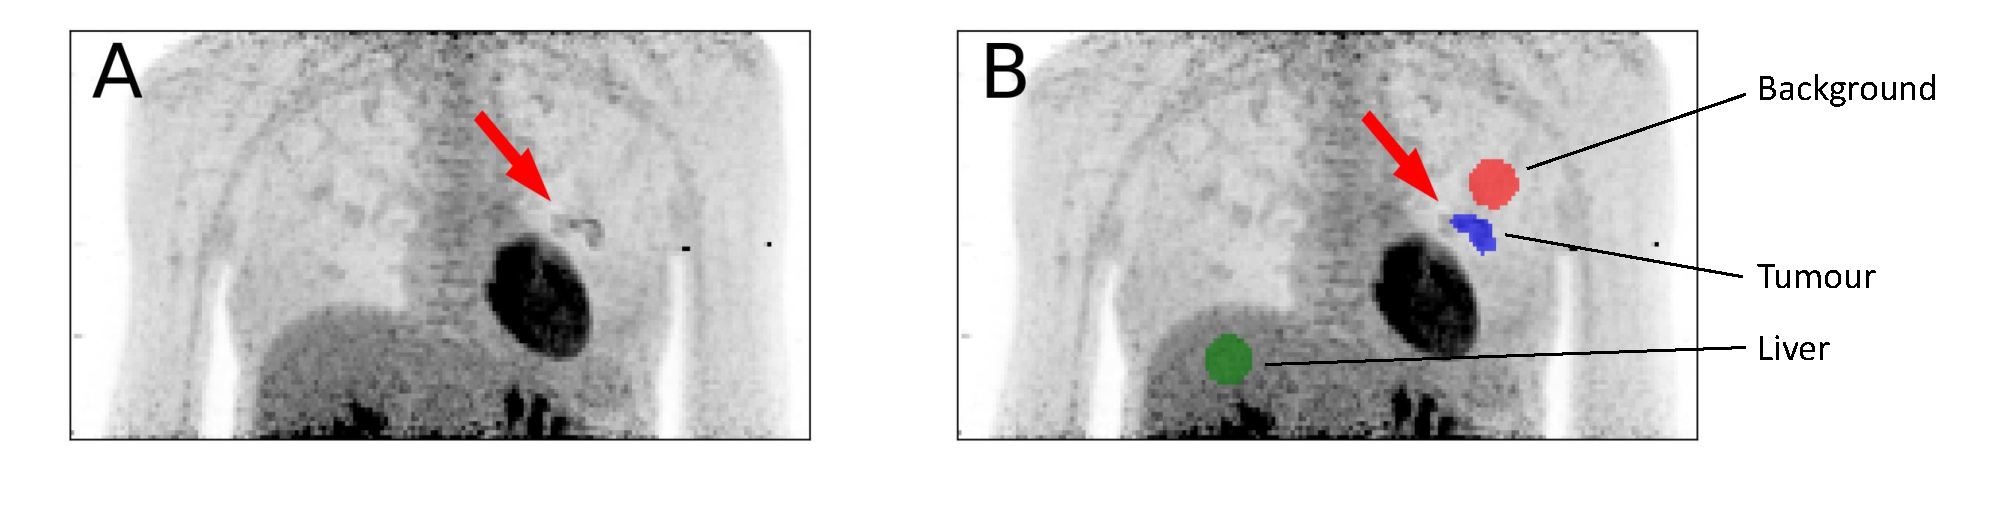
\includegraphics[scale=0.47,angle=0]{3_Results/3_2_Dynamic_Reconstruction_SimulationStudy/figures/RealDataVOIs.pdf}
\caption{Real data MIP SUV image (A) and the drawn VOI (B).}
\label{fig:2_5_VOIs}
\end{figure} 

Similarly, CNR was calculated in a single noise realisation of the simulation study to enable direct comparison with the real data. In this case the eroded thalamus VOI was used as the target region and the white matter as the background for both contrast and noise estimation. 


% Results --------------------------------------------------------------------------------------------
\section*{Results}
 
\subsection*{Comparison between SB and DWB protocol data}
The VOI and voxel based metrics comparing 3D and 4D Patlak reconstructions for the SB and DWB-1 protocols are shown in figure~\ref{fig:3_1_Patlak}. For both metrics and VOIs the 3D reconstruction followed by post-reconstruction Patlak fitting using DWB data resulted in higher CoV values, compared to 3D reconstruction of SB data at matched bias. For the first few iterations the 3D reconstructions of both datasets resulted to similar bias values, while further iterations resulted to a wider range of bias values for the DWB data compared to SB data within 40 iterations.

The use of 4D Patlak reconstruction on DWB data produced results with lower CoV on both evaluated metrics and VOIs, compared to the 3D reconstruction of the same data at matched bias, and a shorter range of bias values within 40 iterations.
For the VOI metrics, CoV values of the 4D Patlak reconstruction on both evaluated regions approach those of 3D reconstruction of SB data. Furthermore, the 4D Patlak reconstruction of DWB data resulted in eroded thalamus bias values that evolved towards a steady value of positive bias, at approximately iteration 12, after which further iterations resulted in small step changes towards lower bias. 
For the voxel metrics, similar behaviour is seen on early iterations of 4D Patlak reconstruction on DWB data for the CoV, with values approaching those of 3D reconstruction of SB data. But at further iterations the CoV for the 4D Patlak reconstruction in both VOIs surpasses values from 3D reconstruction on DWB data. On the eroded thalamus this was the case beyond iteration 24, while for the cortex from iteration 22 and beyond. These results show that there is a risk of increasing parametric image noise, greater than that of 3D reconstructions, when the 4D reconstruction is run at high iterations to achieve more favourable and stable mean VOI behaviour.

The use of 4D Patlak reconstruction with SB data showed similar effects on behaviour for CoV and bias on both metrics, compared to 3D reconstruction of SB data, and resulted in the lowest CoV values for these comparisons.

\begin{figure} [ht!]
\centering
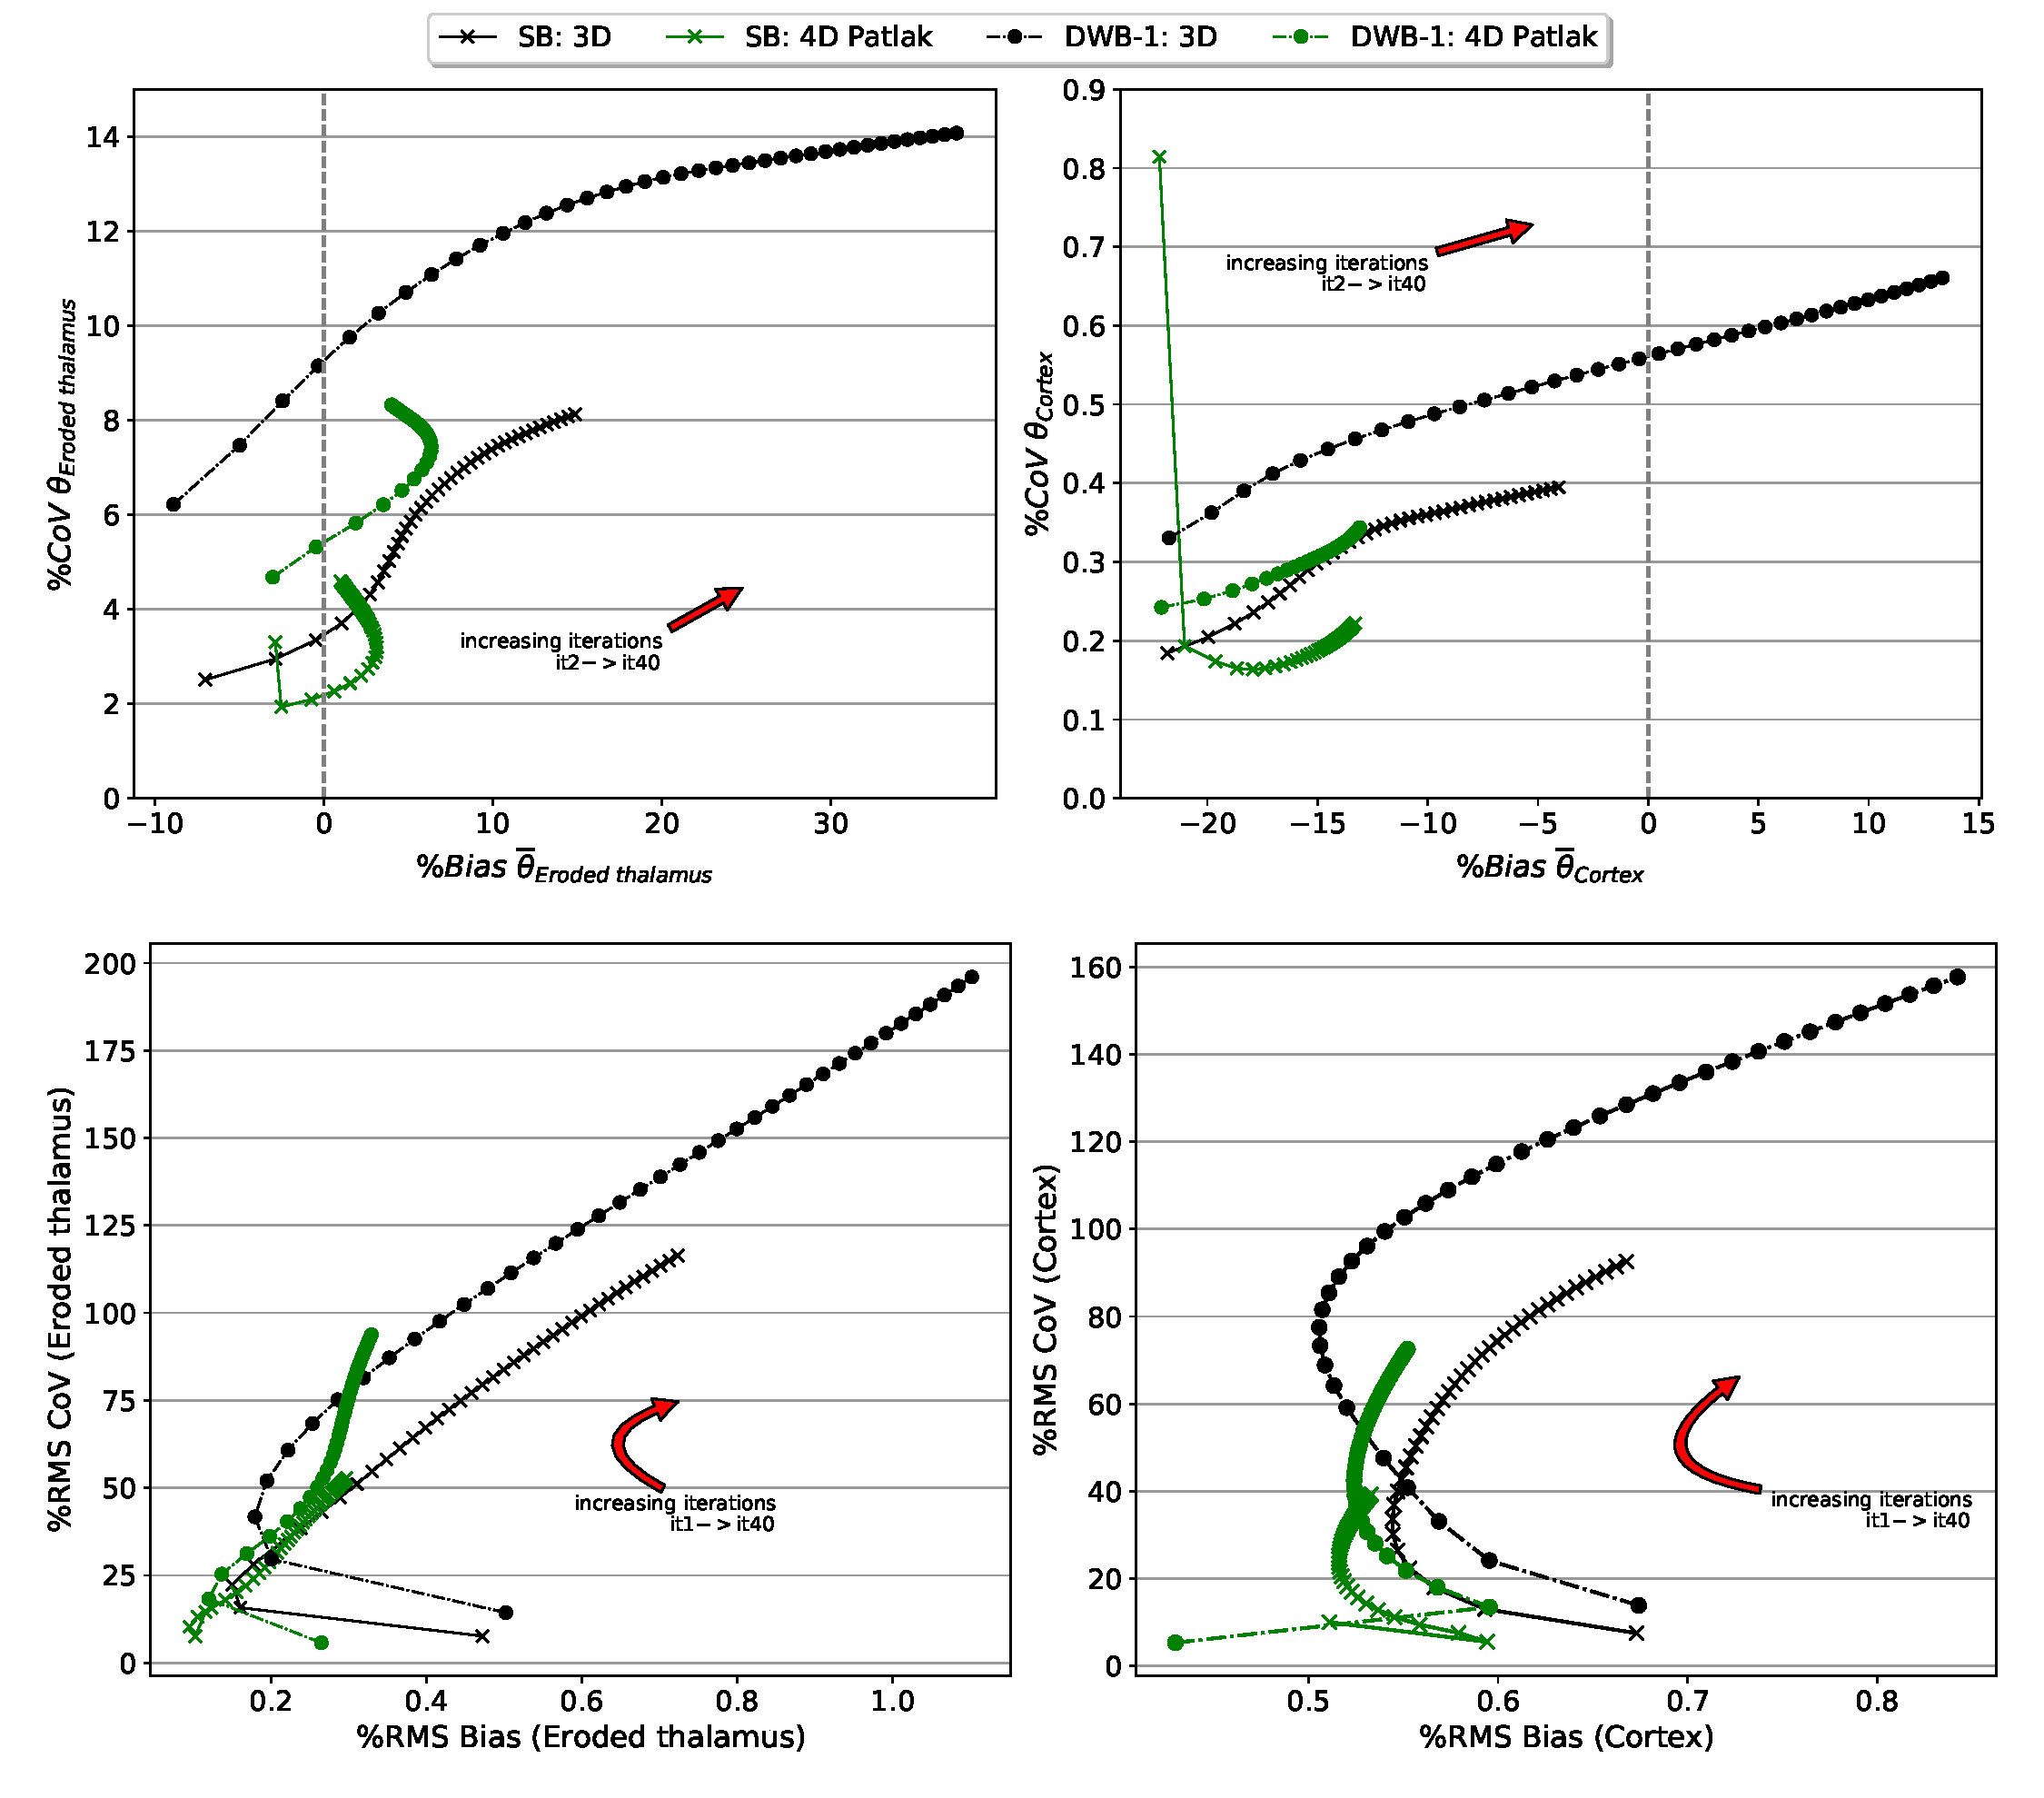
\includegraphics[scale=0.42,angle=0]{3_Results/3_2_Dynamic_Reconstruction_SimulationStudy/figures/VOI/3_1.pdf}
\caption{Simulation: Eroded thalamus (left) and Cortex (right) noise versus bias trade-off curves for 3D and 4D Patlak reconstructions. 
%$K_i$ mean vs. CoV of the mean (top row) and  $K_i$ RMS Bias vs. RMS CoV (bottom row).
VOI based metrics (top row) and voxel-based metrics (bottom row).
}
\label{fig:3_1_Patlak}
\end{figure} 

\subsection*{Comparison between 4D Dynamic Reconstructions on DWB protocol data}
The VOI and voxel based metrics are shown in figure~\ref{fig:3_2_DynamicModels} for comparison of 4D Patlak and 4D Spectral reconstructions of DWB data.
On both metrics and for both regions the use of Spectral reconstruction with 6 basis functions provided the lowest CoV values at matched bias compared to other 4D reconstructions of DWB data and 3D reconstruction of SB data. However 4D Spectral reconstruction with 6 basis also provided the highest bias values in the eroded thalamus. On the cortex the difference on bias metrics was relatively small between all 4D reconstructions.\\
The 4D Spectral reconstruction with 9 and 17 basis functions resulted to similar bias and CoV values at both regions. Their use resulted in lower CoV compared to 4D Patlak reconstruction and 3D reconstruction of SB data, but higher compared to 4D Spectral using 6 basis. Nonetheless, at the eroded thalamus use of 9 and 17 basis provided improved bias values at matched CoV when compared to the use of 6 basis, closer to bias values from 4D Patlak reconstruction.\\
When the 4D Spectral reconstructions were provided with the same data as the 4D Patlak reconstructions (4 frames with $t>t_{ss}$) instead of all data (8 frames for DWB-1), it resulted in a noticeable increase of the CoV values, with very close noise versus bias trade-offs between 6 and 9 basis. Their trade-off curves got closer to the one of the 4D Patlak reconstruction, with lower bias values on both metrics but higher RMS CoV compared to the 4D Patlak reconstruction.


\begin{figure} [ht!]
\centering
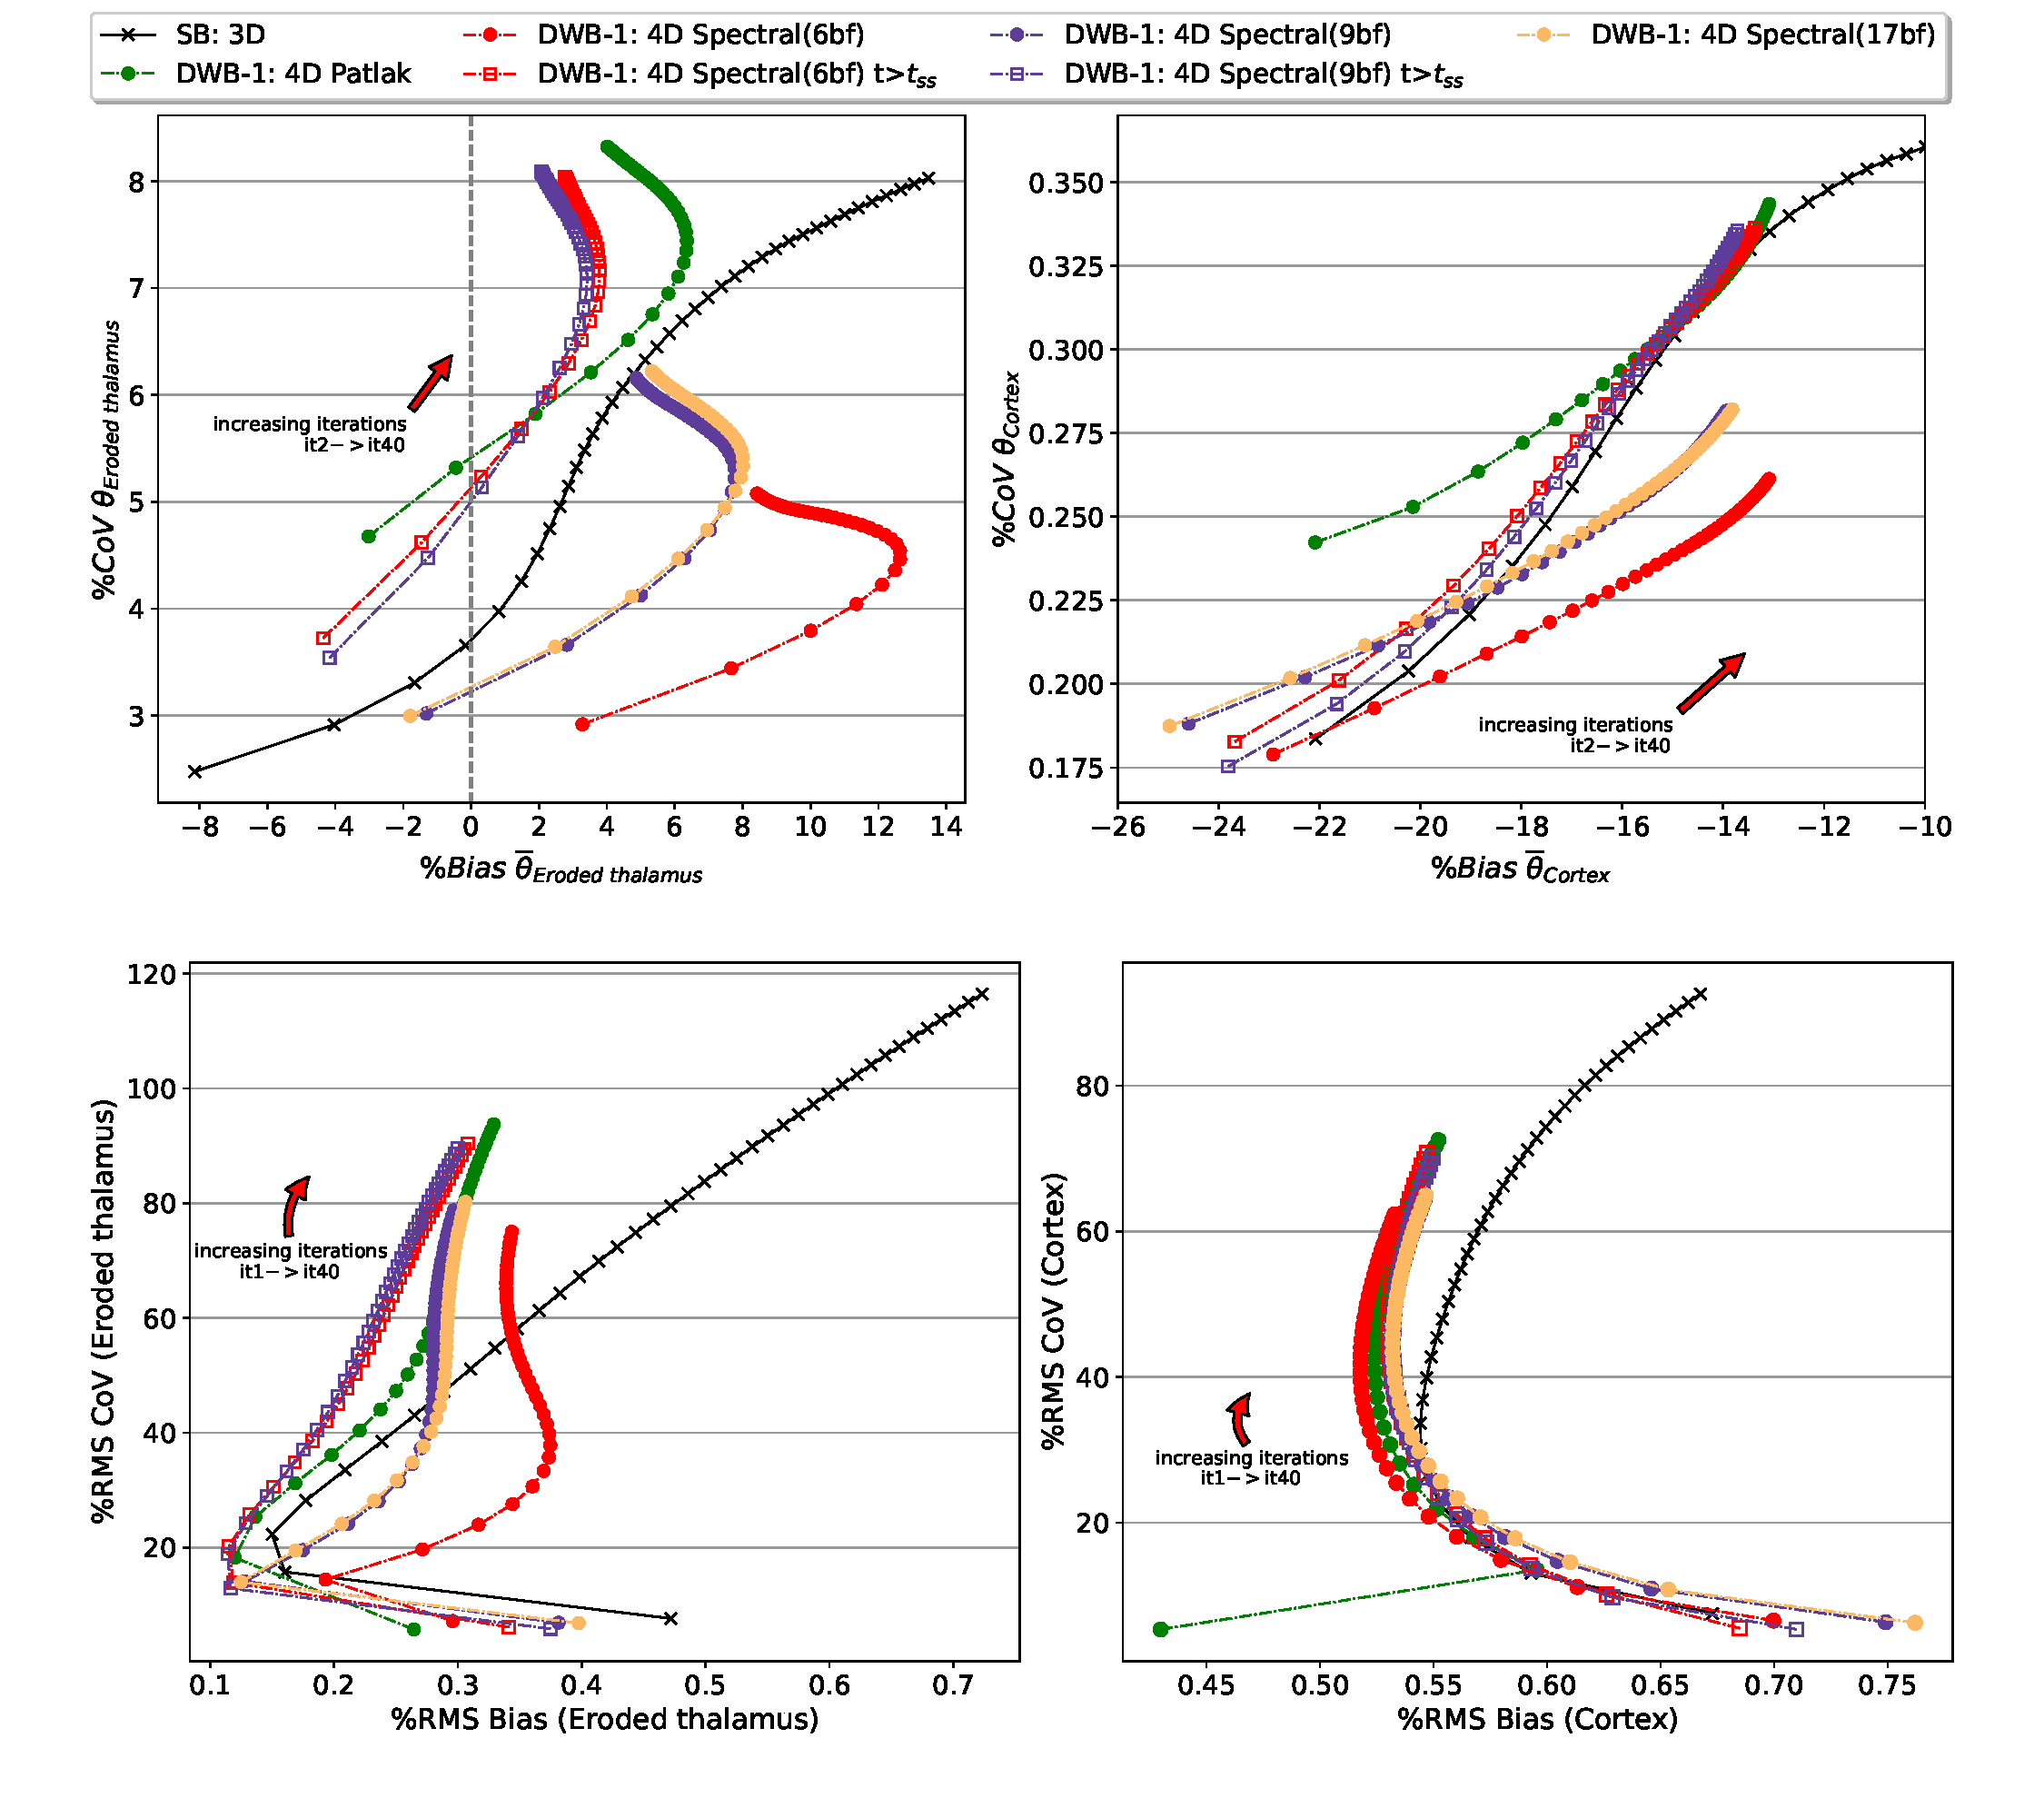
\includegraphics[scale=0.42,angle=0]{3_Results/3_2_Dynamic_Reconstruction_SimulationStudy/figures/VOI/3_2.pdf}
\caption{Simulation: Eroded thalamus (left) and Cortex (right) noise versus bias trade-off curves for 4D reconstructions of DWB-1 protocol data. 
%$K_i$ mean vs. CoV of the mean (top row) and  $K_i$ RMS Bias vs. RMS CoV (bottom row).
VOI based metrics (top row) and voxel-based metrics (bottom row).}
\label{fig:3_2_DynamicModels}
\end{figure} 


\subsection*{Comparing between nested optimizations in 4D reconstruction}
Results of 4D Spectral and 4D Patlak reconstructions using MLEM and NNLS nested optimization are shown in figure~\ref{fig:3_3_DifferentNestedOptimization}. A clear difference in behaviour is seen going from MLEM to NNLS from early iterations, with 4D reconstructions using nested NNLS optimization resulting in higher CoV values at matched bias compared to the respective 4D reconstruction using nested MLEM (with 20 nested sub-iterations). At the same time, NNLS nested optimization often resulted to a slight reduction in bias at matched CoV values.
No difference was seen in convergence properties such as convergence speed between the two nested optimization options. 
Nevertheless the use of a single run of NNLS optimization in each nested loop, instead of 20 nested MLEM iterations, resulted in notable reduction of overall reconstruction times. The average reconstruction times using the two methods on a computer using a 16-core 2.20GHz processor and 96GB of RAM memory are shown in table~\ref{tab:ReconTimes}.

\begin{figure} [ht!]
\centering
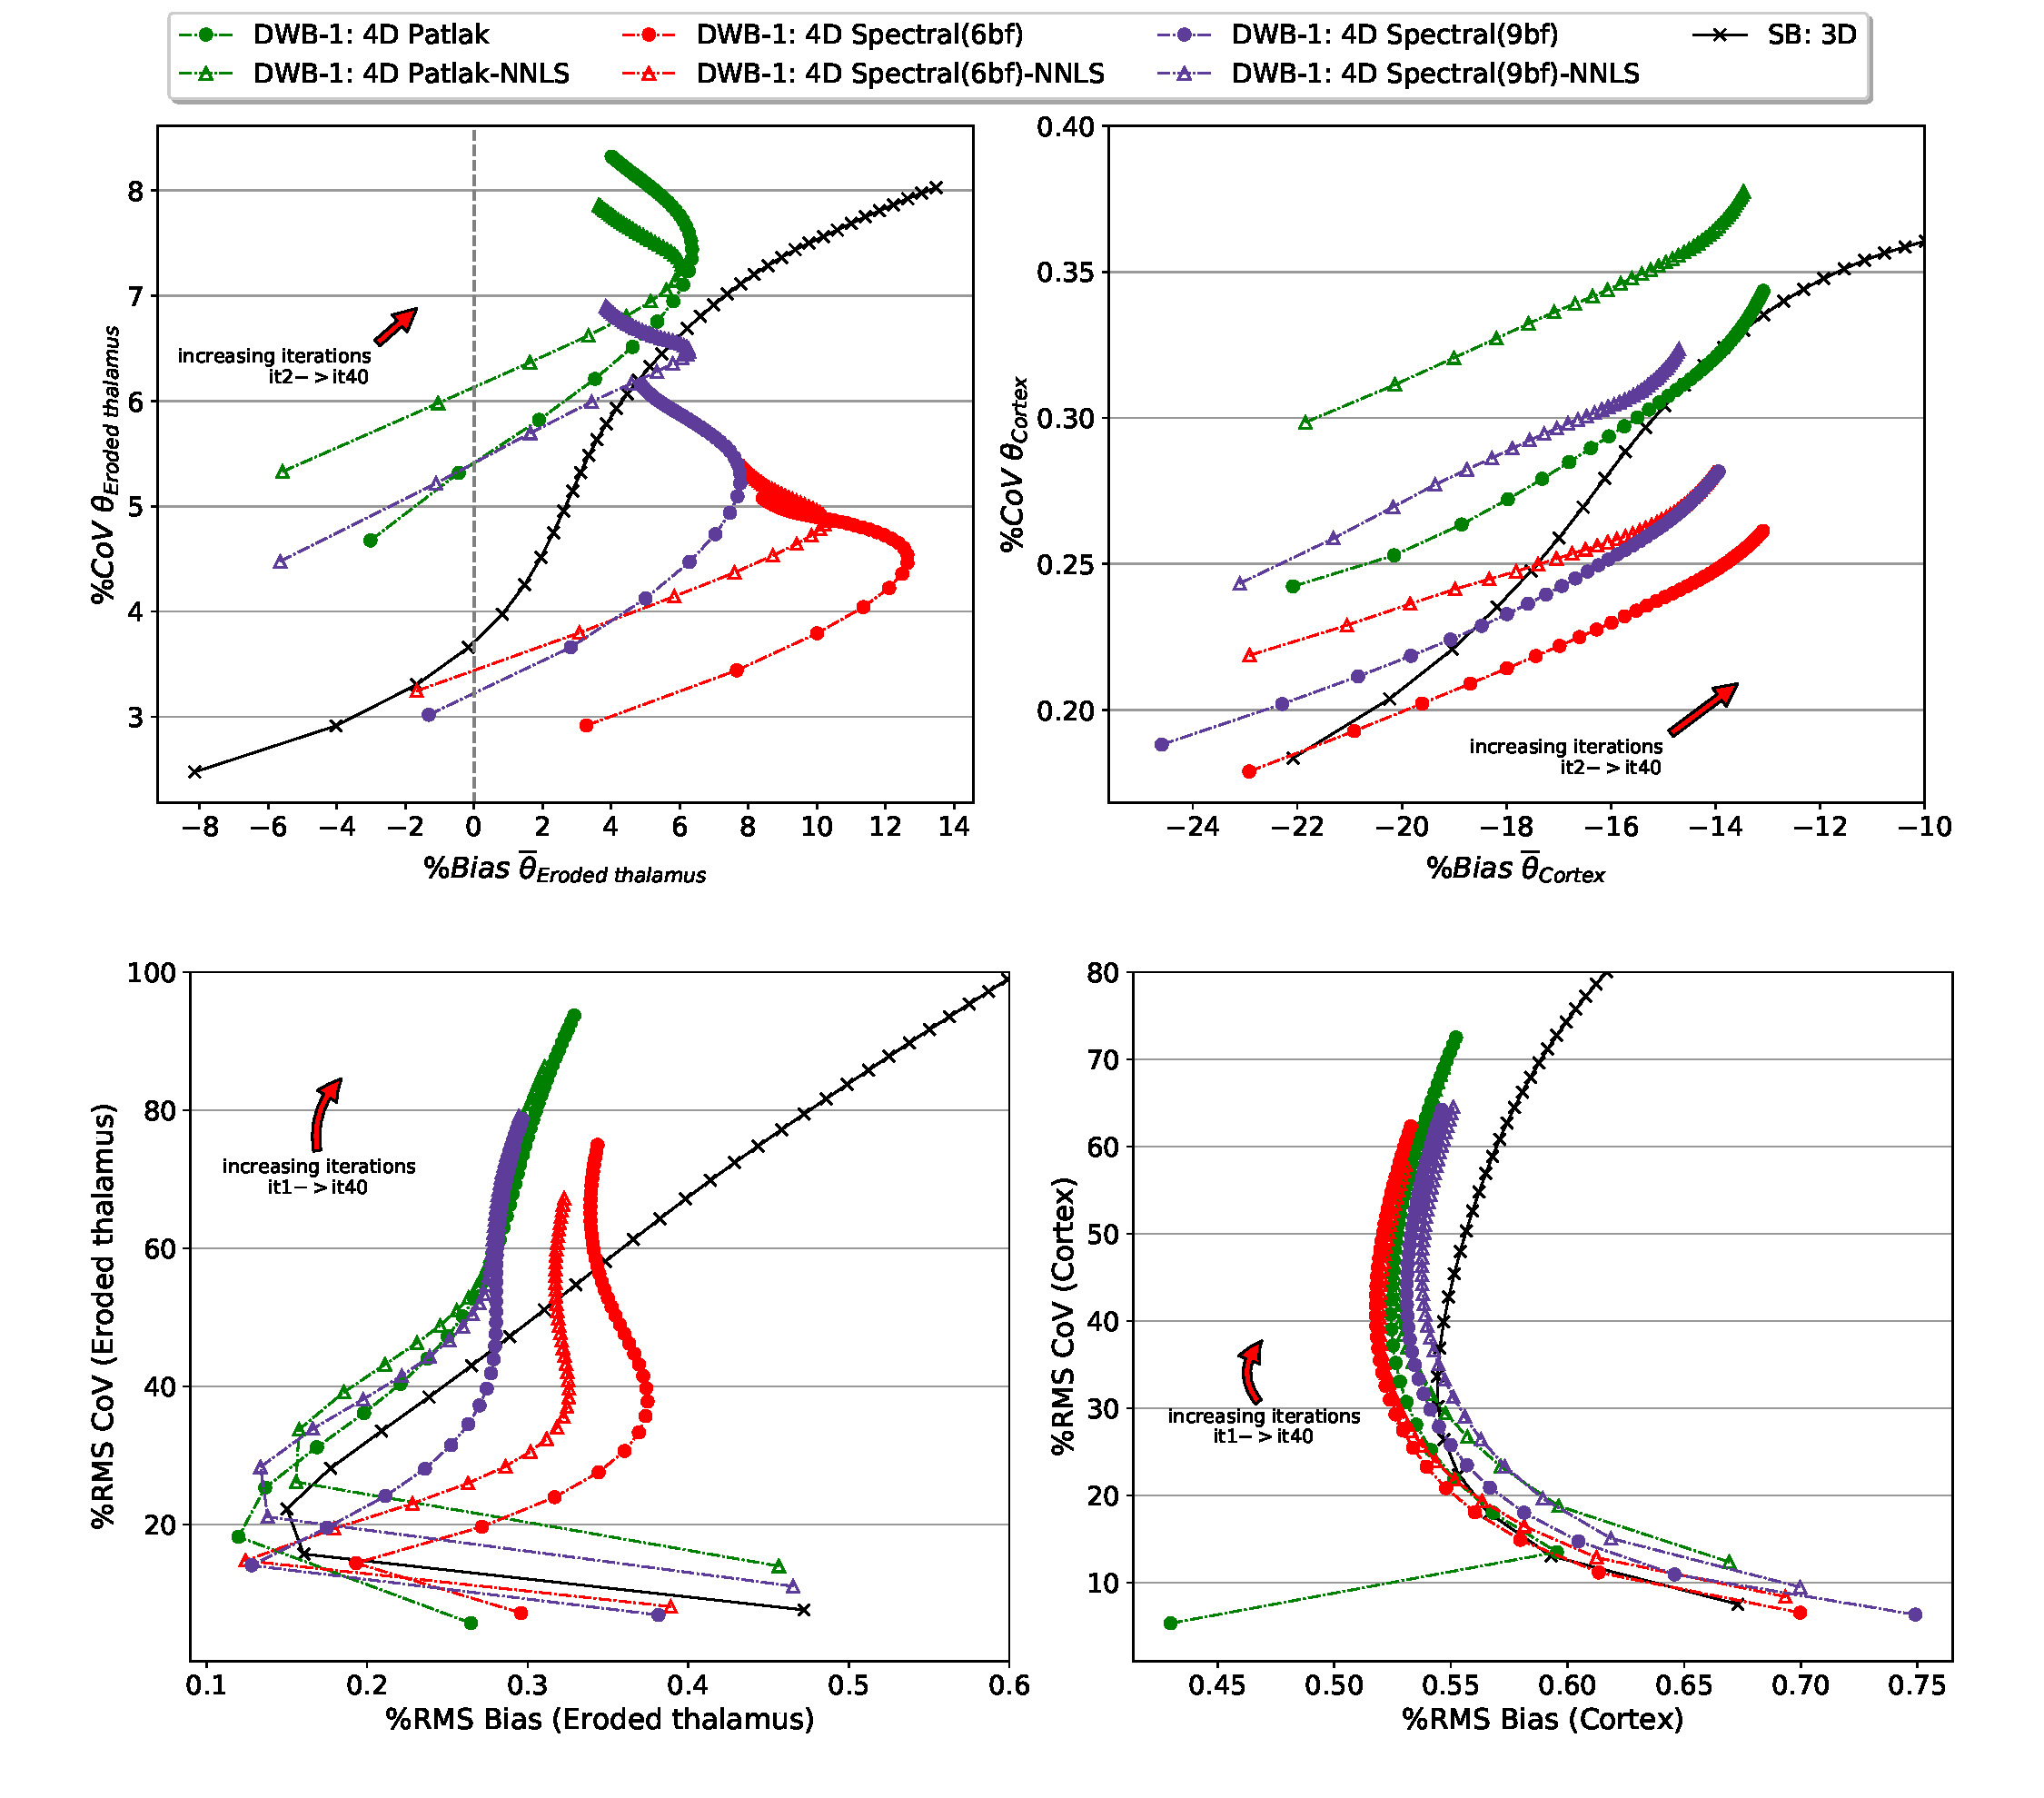
\includegraphics[scale=0.42,angle=0]{3_Results/3_2_Dynamic_Reconstruction_SimulationStudy/figures/VOI/3_3.pdf}
\caption{Simulation: Eroded thalamus (left) and Cortex (right) noise versus bias trade-off curves for 4D reconstructions, with MLEM and NNLS nested optimization. VOI based metrics (top row) and voxel-based metrics (bottom row).} 
\label{fig:3_3_DifferentNestedOptimization}
\end{figure} 
% Simulation: Eroded thalamus $K_i$ RMS Bias vs. RMS CoV for 4D reconstructions, with MLEM and NNLS nested optimization

\begin{table}[h!]
\centering
\caption{\label{tab:ReconTimes}Average reconstruction times for 1 full iteration (28 subsets) over DWB-1 data using CASToR.}
\begin{tabular}{lll}
\toprule
\textbf{Reconstruction} & \textbf{nested MLEM (min)} & \textbf{nested NNLS (min)} \\ 
\midrule
4D Patlak               & 9.6  & 6.7  \\
4D Spectral(6bf)        & 14.0 & 8.2  \\   
4D Spectral(9bf)        & 15.8 & 8.3  \\ 
4D Spectral(17bf)       & 26.6 & 11.2 \\
\toprule
\end{tabular}
\end{table}

\subsection*{Comparison between DWB protocols}
Comparison of 4D Patlak and 4D Spectral reconstructions between the three simulated DWB protocols is made in figure~\ref{fig:3_4_ComparingDWBProtocols}. For both VOI regions and 4D reconstructions, data from all three DWB protocols resulted in close bias values at matched iteration number, with a slight deviation in RMS bias towards late iterations.
Differences in CoV at matched bias values are more profound in VOI metrics of the cortex region, where data from protocol DWB-2 resulted in the lowest CoV values and DWB-1 and DWB-3 data resulted to closer CoV values. This level of reduction in CoV was not seen on the eroded thalamus, neither on VOI or voxel based metrics. In the eroded thalamus the differences of DWB protocols on CoV at matched  bias were smaller and their ordering was mixed between the two 4D reconstructions. 

\begin{figure} [ht!]
\centering
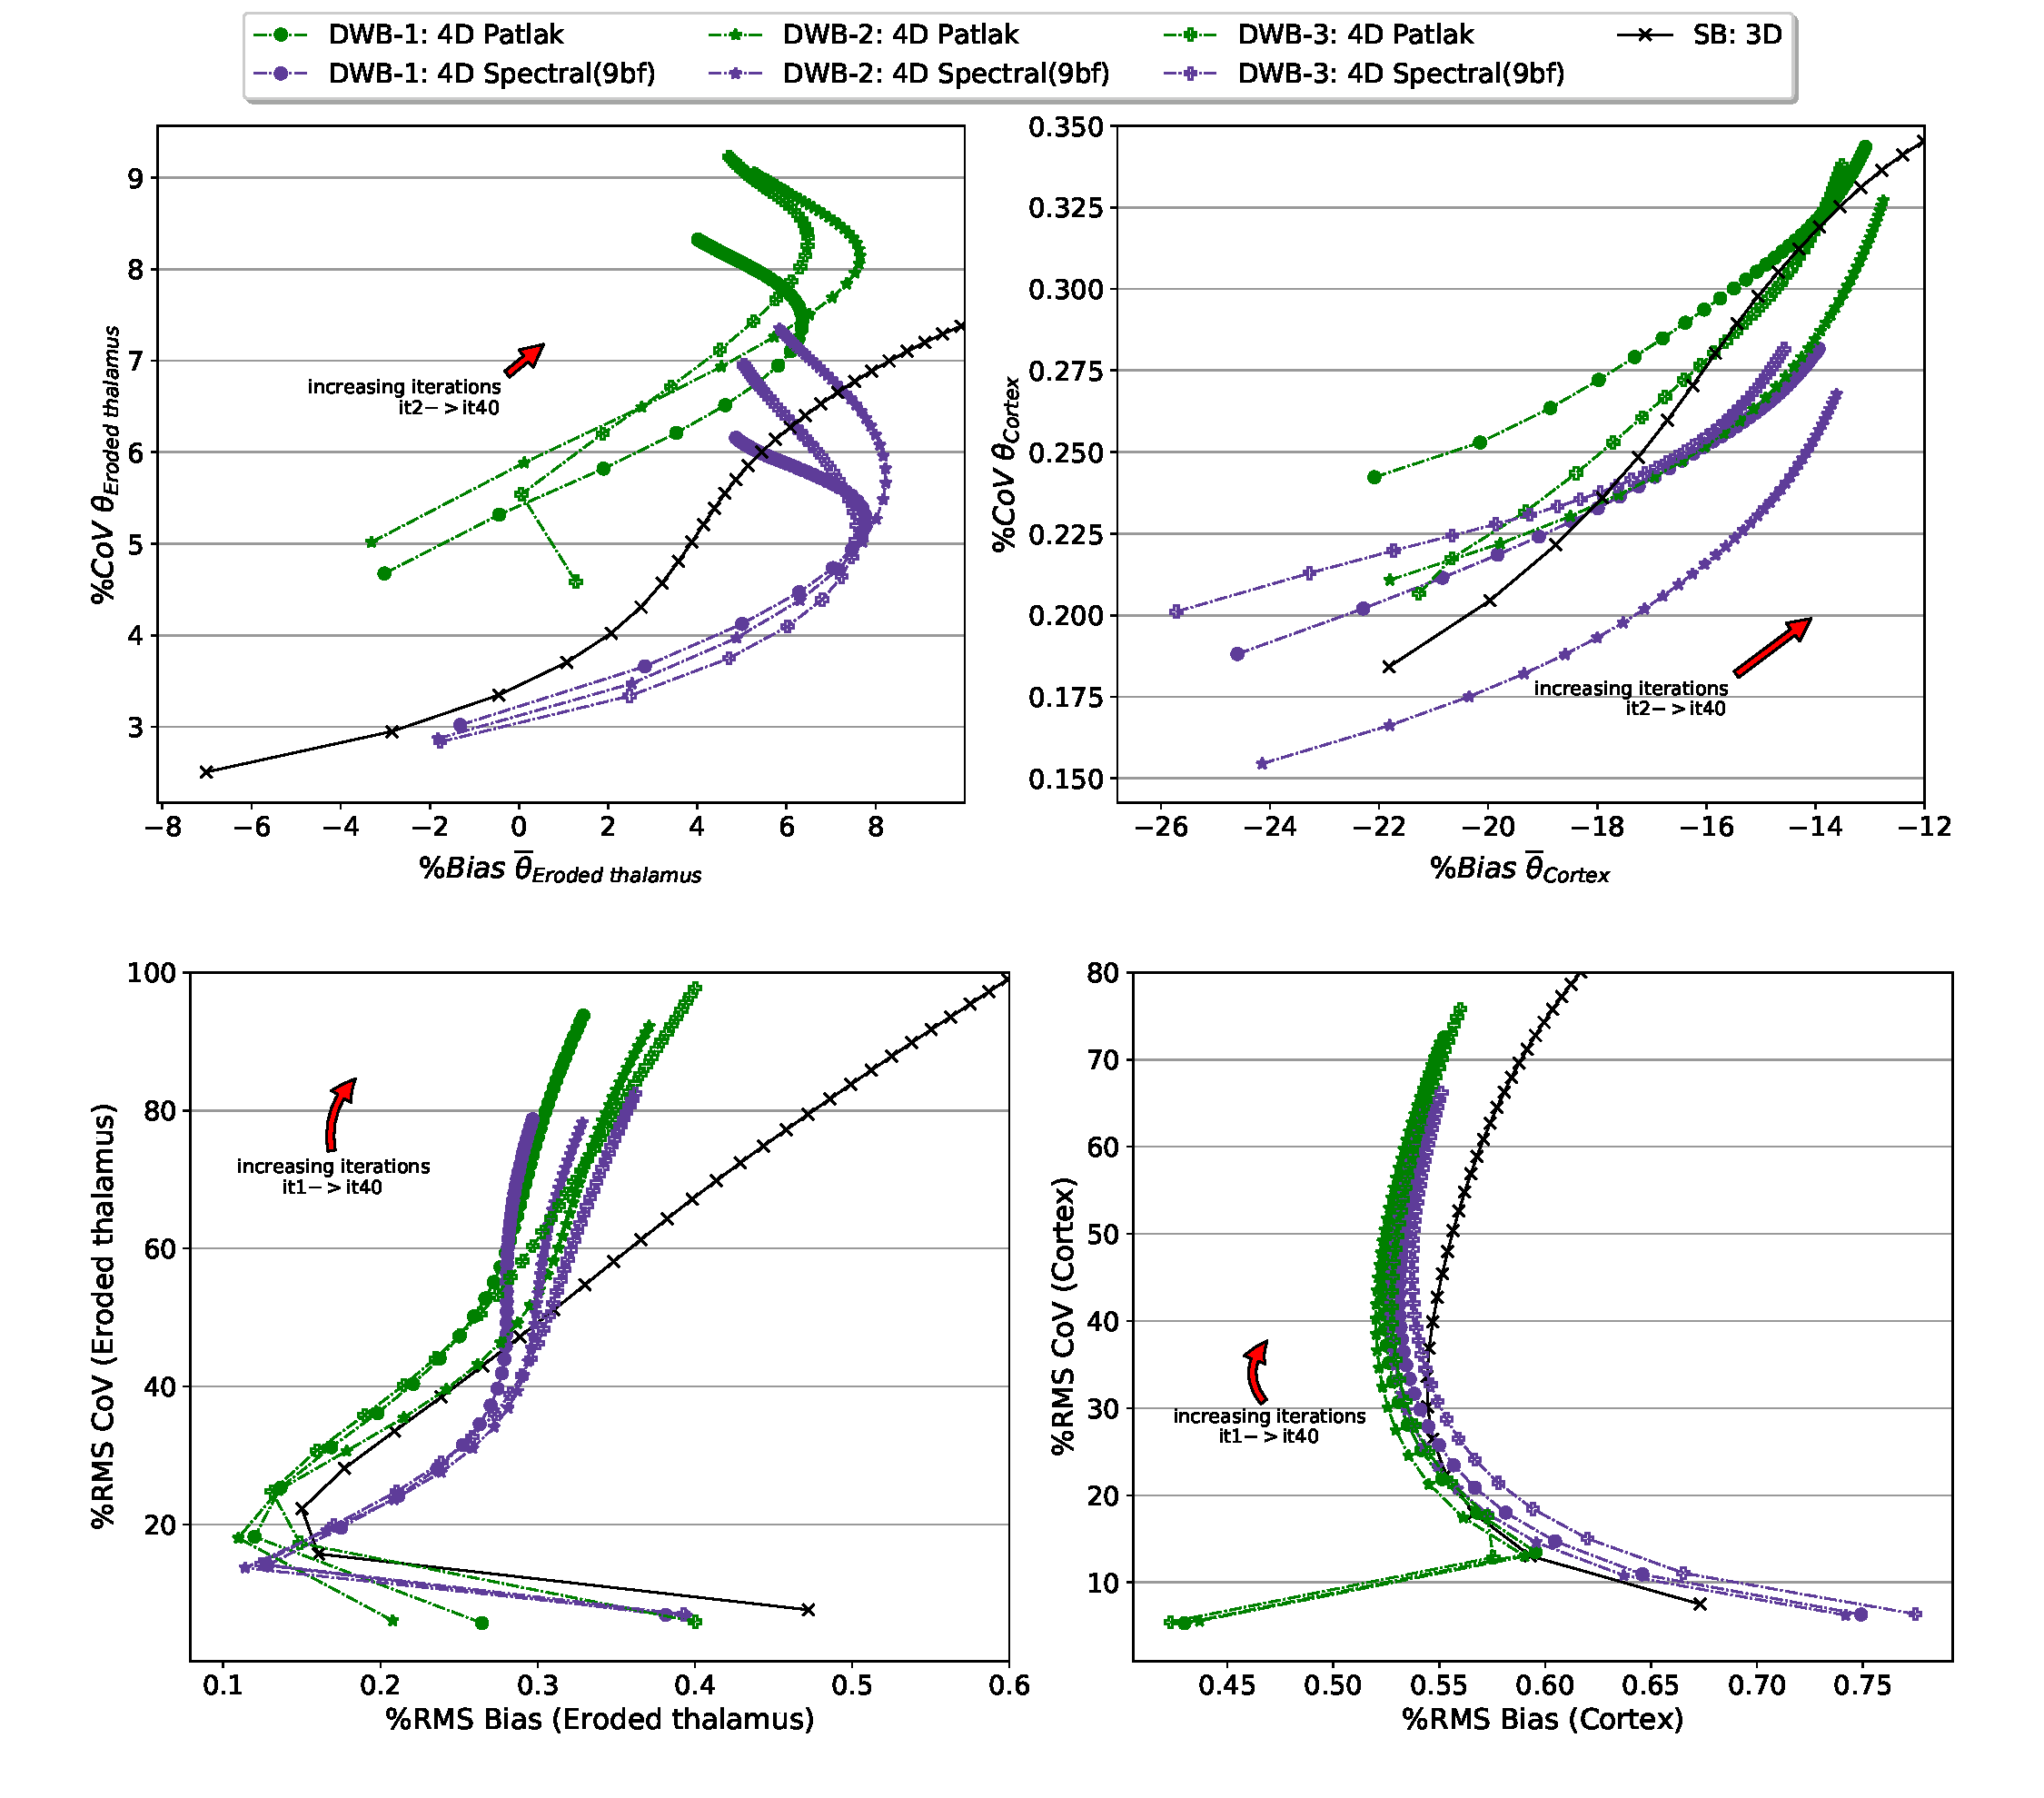
\includegraphics[scale=0.42,angle=0]{3_Results/3_2_Dynamic_Reconstruction_SimulationStudy/figures/VOI/3_4.pdf}
\caption{Simulation: Eroded thalamus (left) and Cortex (right) noise versus bias trade-off curves for 4D reconstructions of the simulated DWB protocol data. VOI based metrics (top row) and voxel-based metrics (bottom row).} 
\label{fig:3_4_ComparingDWBProtocols}
\end{figure} 
%Simulation: Eroded thalamus $K_i$ RMS Bias vs. RMS CoV for 4D Patlak and 4D Spectral reconstructions of the simulated DWB protocol data

\subsection*{Comparison with real data}
The comparison of reconstructions using a real FDG dataset, reprocessed and reconstructed with the SB and DWB-1 protocol framings, is made in figure~\ref{fig:RealData_CNR_CoVBias_NoTOF} for non-TOF reconstructions and in figure~\ref{fig:RealData_CNR_CoVBias} for reconstructions using TOF. %A similar comparison is made with simulated data in figure~\ref{fig:3_2_SingleReplicateMeanCov} for one randomly chosen noise replicate of DWB-1.
Results on the real data showed similar evolution of CNR with increasing iterations for 4D and 3D reconstructions, for non-TOF and TOF reconstructions respectively.
The 4D Spectral reconstruction using 6 basis functions provided the highest CNR values throughout all iterations, followed by the 4D Spectral reconstruction using 9 basis functions and 4D Patlak. Overall, CNR of all 4D reconstructions of DWB data was higher than that of 3D reconstruction of SB data and 3D reconstruction of DWB data.\\
The tumour SD vs VOI average trade-off curves showed close behaviour between 4D reconstructions using TOF, resulting to SD values in the first 15 to 17 iterations of 4D reconstructions which were lower compared to 3D reconstruction of DWB data at matched tumour mean values. Compared to 3D reconstruction of SB data, all 4D reconstructions of DWB data resulted in higher SD values (for matched tumour mean values where comparison is possible).
For 4D reconstructions of DWB data without TOF information, tumour SD values were lower to 3D reconstruction of DWB data for the first 16 to 25 iterations, while higher than 3D reconstructions of SB data at matched mean tumour values. 
\textcolor{blue}{Mean tumour $K_i$ values were lower in reconstructions without TOF compared to all reconstructions using TOF at respective 3D and 4D reconstructions. The difference was also seen in VOI TAC measurements of the tumour between non-TOF and TOF 3D reconstructions and can be attributed to differences in contrast recovery within the reconstruction by use of TOF information.}

Parametric $K_i$ images from 3D and 4D reconstructions with TOF at iterations with matched liver SD values of approximately 4$\cdot$10$^{-3}$~min$^{-1}$ are shown in figure~\ref{fig:RealKiMontage}.

\begin{figure} [ht!]
\centering
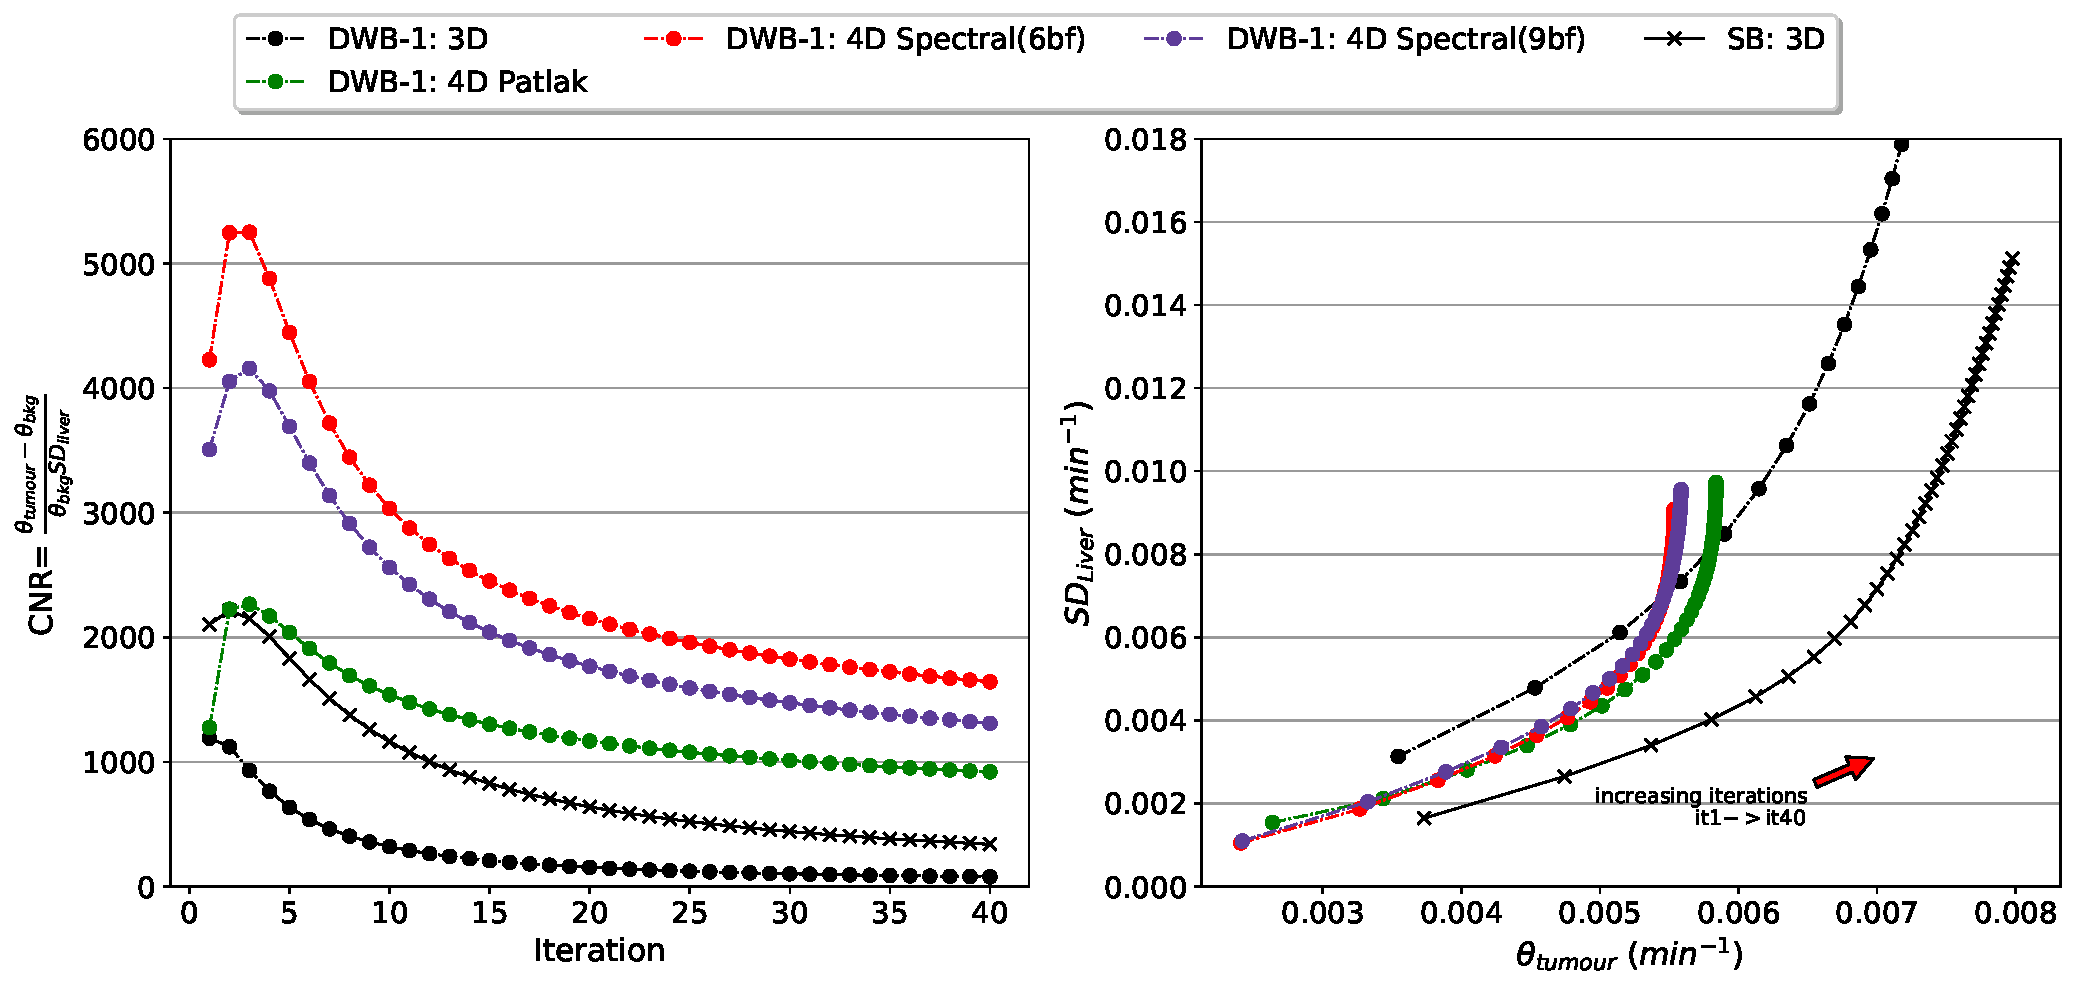
\includegraphics[scale=0.45,angle=0]{3_Results/3_2_Dynamic_Reconstruction_SimulationStudy/figures/RealData/3_5_tumour_Lung_NoTOF.pdf}
\caption{Real Data: Contrast to Noise ratio (left) and liver SD vs. VOI mean of the tumour (right) for 3D and 4D reconstructions without TOF information.} 
\label{fig:RealData_CNR_CoVBias_NoTOF}
\end{figure} 

\begin{figure} [ht!]
\centering
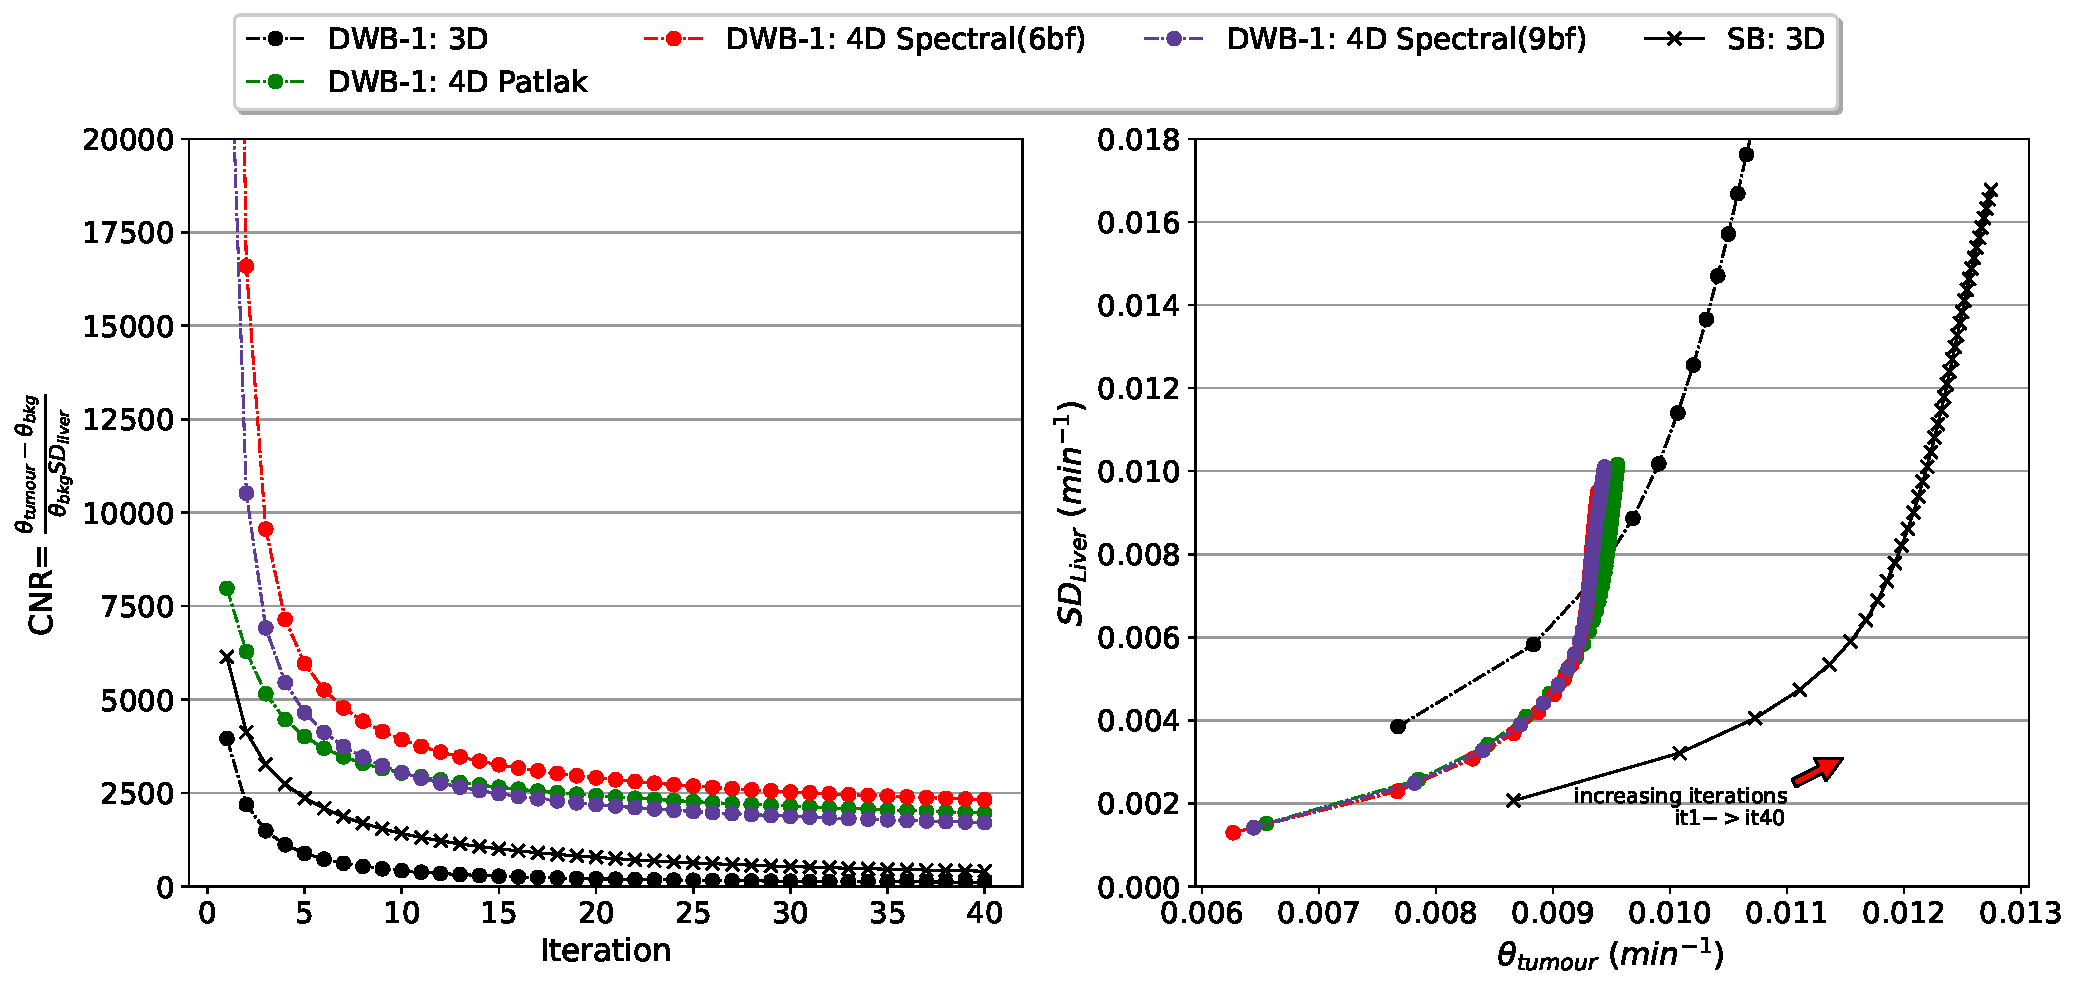
\includegraphics[scale=0.45,angle=0]{3_Results/3_2_Dynamic_Reconstruction_SimulationStudy/figures/RealData/3_5_tumour_Lung.pdf}
\caption{Real Data: Contrast to Noise ratio (left) and liver SD vs. VOI mean of the tumour (right) for 3D and 4D reconstructions using TOF information.} 
\label{fig:RealData_CNR_CoVBias}
\end{figure} 

\begin{figure} [h!]
\centering
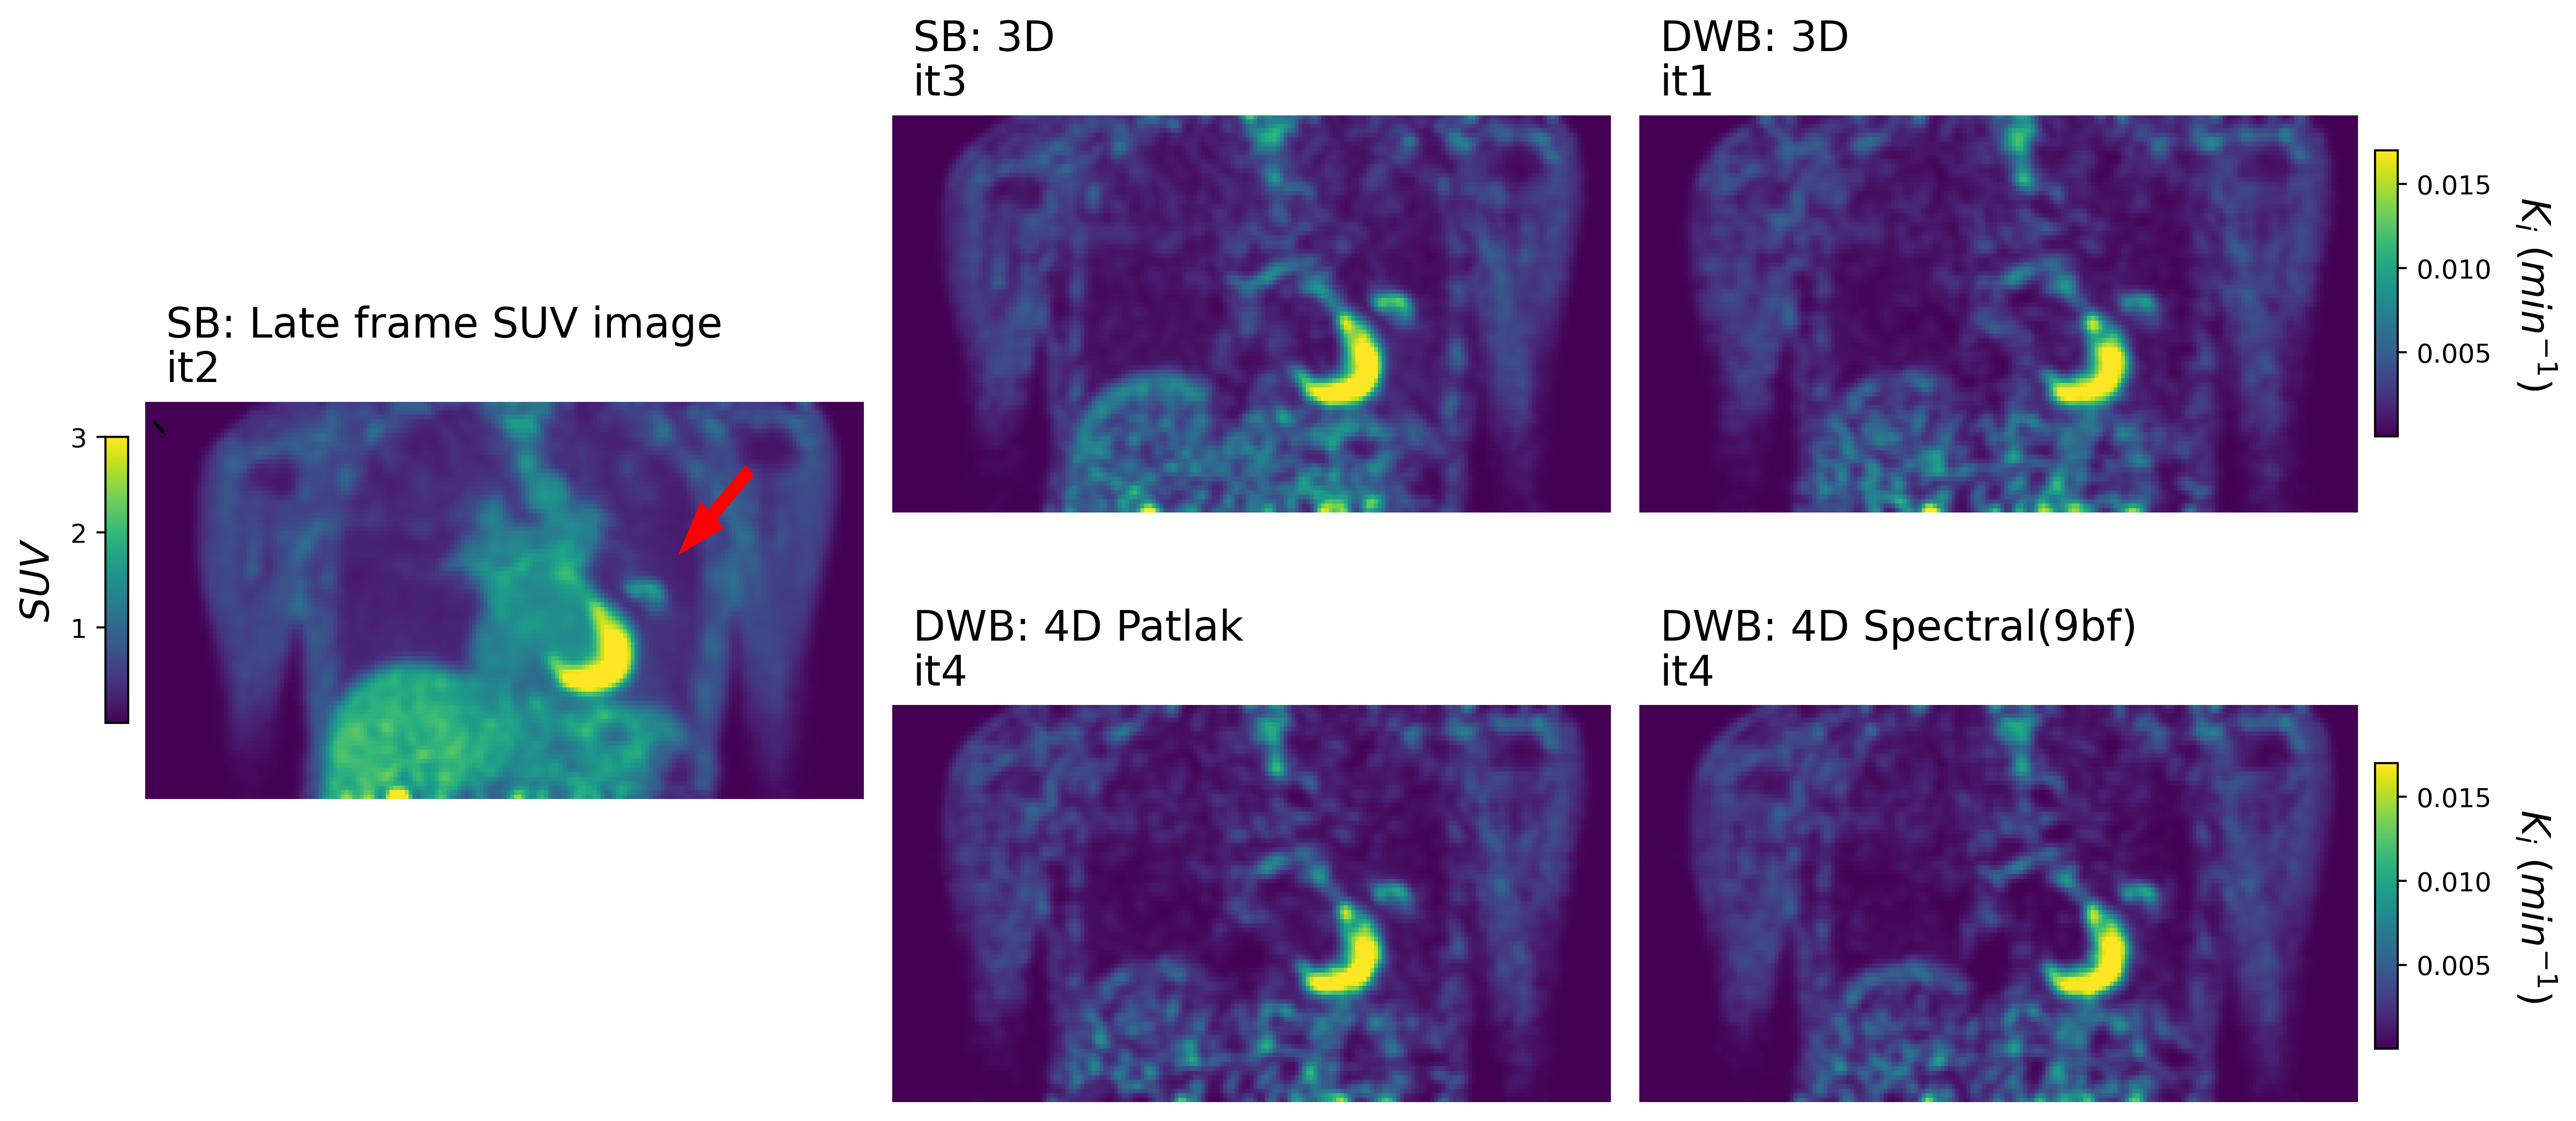
\includegraphics[scale=0.28,angle=0]{3_Results/3_2_Dynamic_Reconstruction_SimulationStudy/figures/RealData/3_5_RealDataExample.png}
\caption{Real Data: Parametric $K_i$ images (with 5mm Gaussian Filtering) from SB and DWB replay datasets from 3D and 4D reconstructions, using TOF information, at matched SD values over the liver.} 
\label{fig:RealKiMontage}
\end{figure} 

For comparison against the simulation study, metrics of CNR and SD vs VOI average trade-off curves from a randomly chosen noise replicate of simulation DWB-1 are shown in figure~\ref{fig:3_2_SingleReplicateMeanCov}.
%\textcolor{blue}{In this dataset a clearer separation between 4D reconstruction algorithms is seen on all plotted metrics.}
\textcolor{blue}{Similarly to the real data, with or without TOF information, values of CNR are highest for 4D Spectral reconstruction using 6 basis functions followed by 4D Spectral reconstruction using 9 basis functions.
For the simulation data and real data without TOF, 4D Patlak reconstruction provided lower CNR values compared to 4D Spectral reconstruction using 9 basis functions and closer to the values of 3D reconstruction from SB data at initial iterations. By contrast, real data using TOF resulted in similar CNR values to those of 4D Spectral reconstruction using 9 basis functions.
Evolution of CNR with increasing iterations was similar between non-TOF real data and simulated data, with maximum values attained between 3 and 5 iterations for all reconstructions.
For real data with TOF, maximum values were attained from the very first iteration while the onward trend with increasing iterations was similar to the non-TOF data for iterations numbers beyond the maximum CNR value was attained.
The difference between the non-TOF and TOF datasets could potentially be attributed to different convergence behaviour due to use of TOF information in the reconstructions of the real data. Differences between the simulation and real data non-TOF reconstructions in absolute values of maximum CNR can be attributed to the different nature of the VOIs used for the respective CNR values.
Finally, the simulation data SD vs VOI average trade-off curves of the eroded thalamus showed separation of 4D reconstructions, with 4D Spectral reconstructions providing lower SD values compared to 3D and 4D Patlak reconstruction of DWB data, but at higher bias values as shown previously in the analysis of simulation results.
Parametric $K_i$ images of 3D and 4D reconstructions at matched RMS CoV values, of approximately 32\% as measured at the eroded thalamus VOI, are shown in figure~\ref{fig:cuts_bias_matched_rms_CoV} for a single noise replicate along with images of mean bias over noise replicates. The single replicate images show that structures of the thalamus seen in 3D reconstruction of SB data are better resolved in DWB when using the 4D Spectral reconstruction. The images of bias show similar behaviour in the thalamus over reconstructions and demonstrate the partial volume effects at the cortex region.}

\begin{figure} [ht!]
\centering
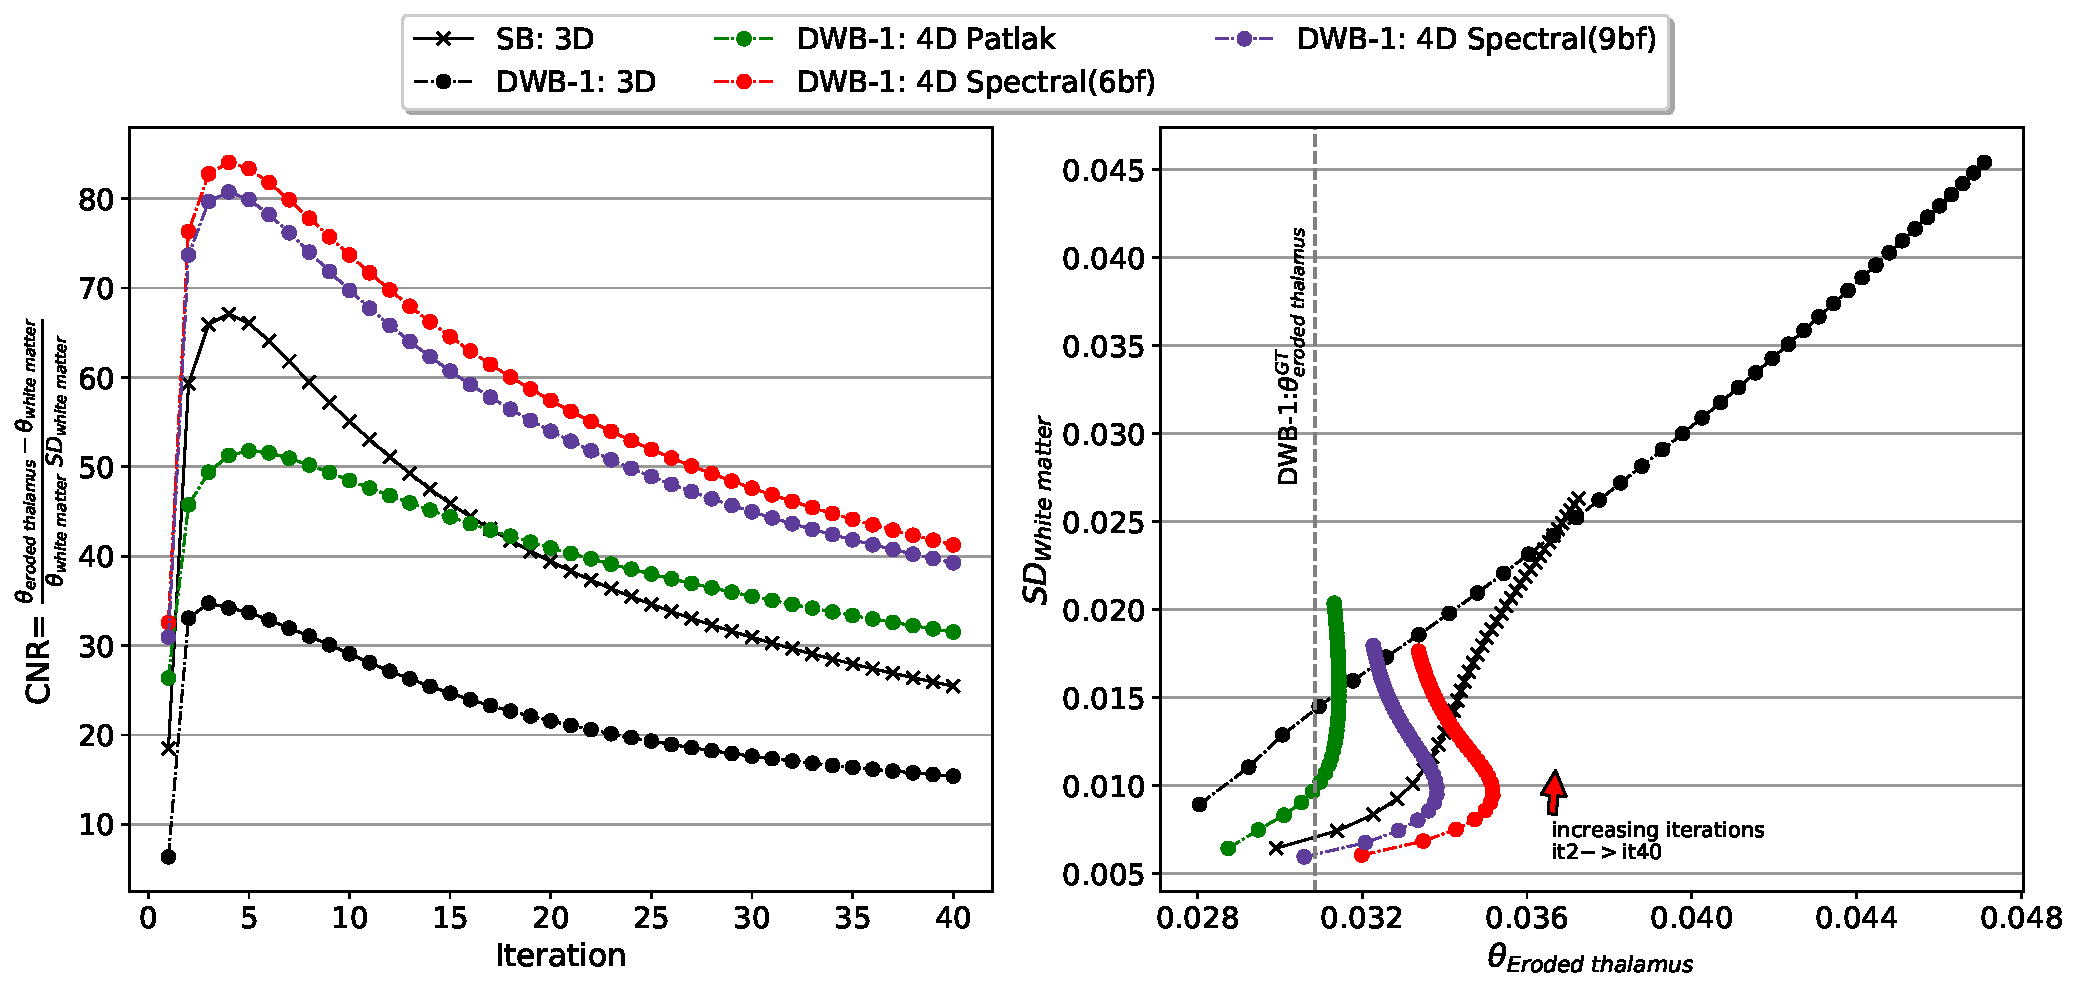
\includegraphics[scale=0.45,angle=0]{3_Results/3_2_Dynamic_Reconstruction_SimulationStudy/figures/Single/3_8_SingleReplicate.pdf}
\caption{Simulation single noise realisation of DWB-1 data: Contrast to Noise ratio (left) and white matter SD vs. eroded thalamus $K_i$ mean for 3D and 4D reconstructions.} 
\label{fig:3_2_SingleReplicateMeanCov}
\end{figure} 

\begin{figure} [h!]
\centering
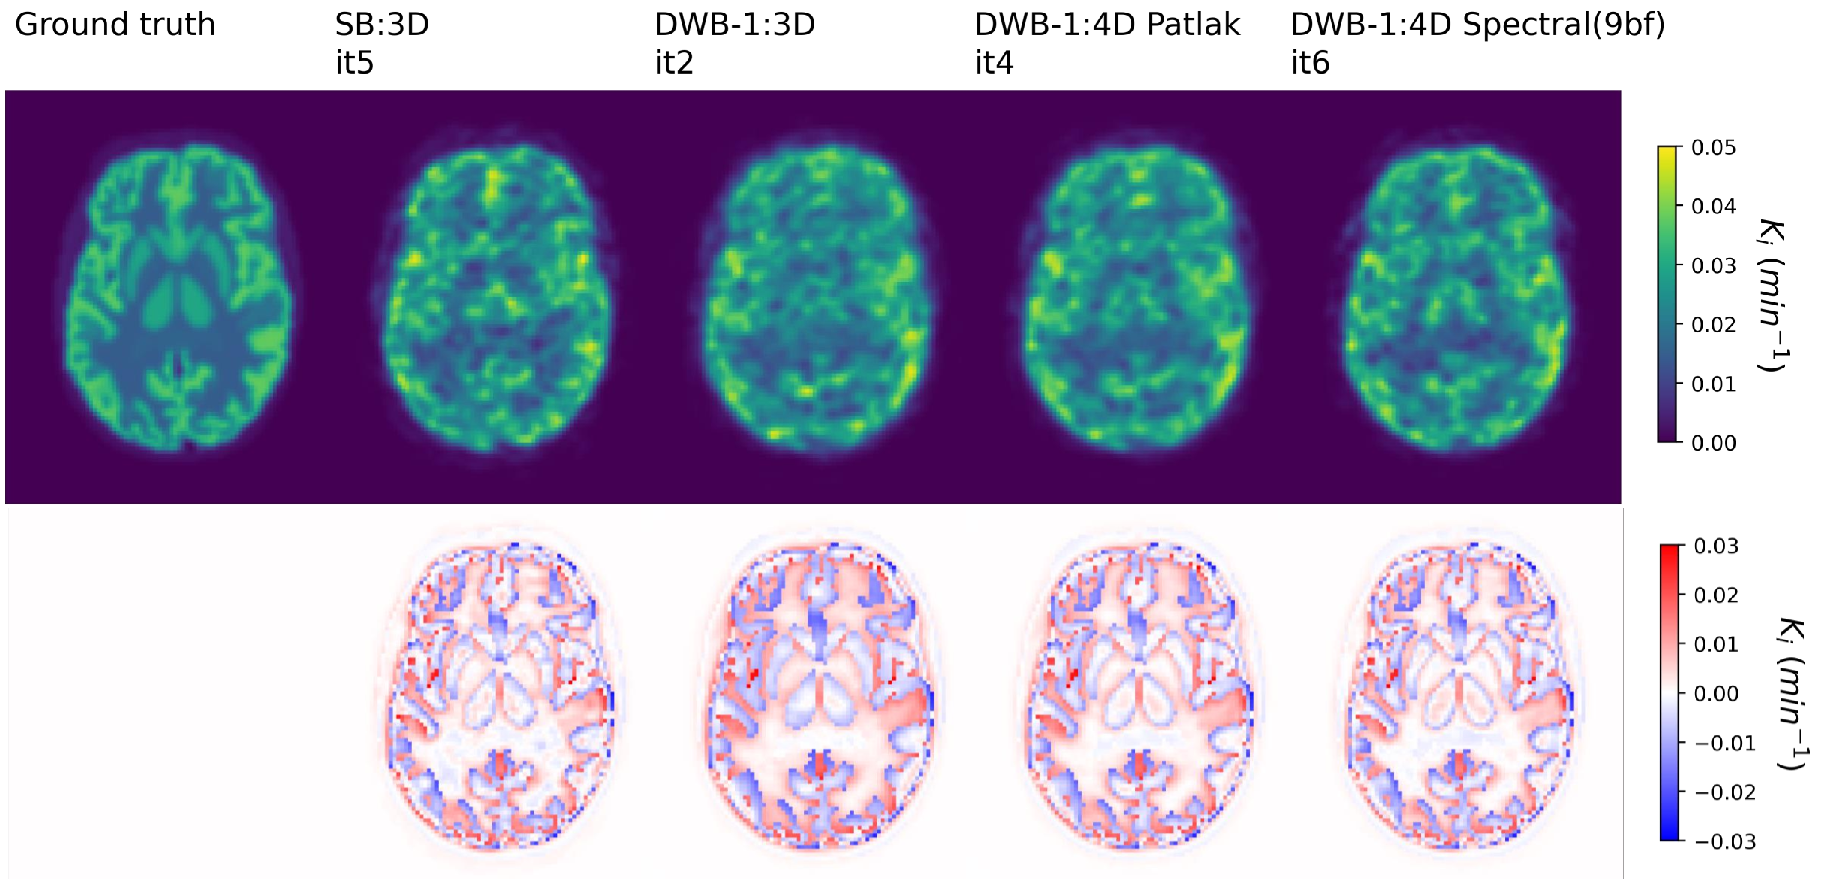
\includegraphics[scale=0.47,angle=0]{3_Results/3_2_Dynamic_Reconstruction_SimulationStudy/figures/BrainCuts/BrainCuts.pdf}
\caption{Single slice though parametric $K_i$ images of one noise replicate (with 3mm Gaussian Filtering) (top) and their corresponding Bias images (over noise replicates) (bottom) from SB and DWB data 3D and 4D reconstructions at matched RMS CoV in the eroded thalamus.}
\label{fig:cuts_bias_matched_rms_CoV}
\end{figure} 

\subsection*{Parametric \boldsymbol{$K_1$} imaging from 4D Spectral reconstruction}
\textcolor{blue}{
The VOI and voxel based metrics for parametric $K_1^*$ images from the SB, DWB-1 and DWB-4 protocols are shown in figure~\ref{fig:K1_WB1} and figure~\ref{fig:K1_SB_WB4}. For the results from DWB-1 the missing fast dynamic data in the early minutes of the acquisition results in erroneous bias and noise levels on both VOI and voxel based metrics. By contrast, the results from the DWB-4 protocol which makes use of the single bed dynamic acquisition along with the DWB acquisition resulted in VOI and RMS mean similar to that of the SB protocol. For both protocols results show overestimation of mean VOI measurements in the eroded thalamus VOI and underestimation in the cortex VOI. It is important to note here that the ignored blood fraction correction in parametric $K_1^*$ images contributes towards an approximate 3\% negative bias in quantification, if we consider the simulated blood fraction of 0.03 in the thalamus and cortex regions.
Measurements of RMS CoV show that data from the DWB-4 protocol result in higher noise compared to SB protocol.
Parametric $K_1^*$ images of the evaluated acquisition protocols at matched RMS CoV values, of approximately 40\% as measured at the eroded thalamus VOI, are shown in figure~\ref{fig:K1_cuts_bias_matched_rms_CoV} for a single noise replicate along with images of mean bias over noise replicates. The images from the single replicates of SB and DWB-4 protocol data show similar structures and contrast of these structures, in comparison to the contrast of the ground truth values. The DWB-1 data show the erroneous overestimation of the values and loss of contrast between structures. This is also seen in the bias images for the DWB-1 data, while the bias structures in DWB-4 and SB data are very similar and closer to zero bias. The images of bias demonstrate the effect of partial volume effects, similarly to the effects shown for $K_i$.}

\begin{figure} [ht!]
\centering
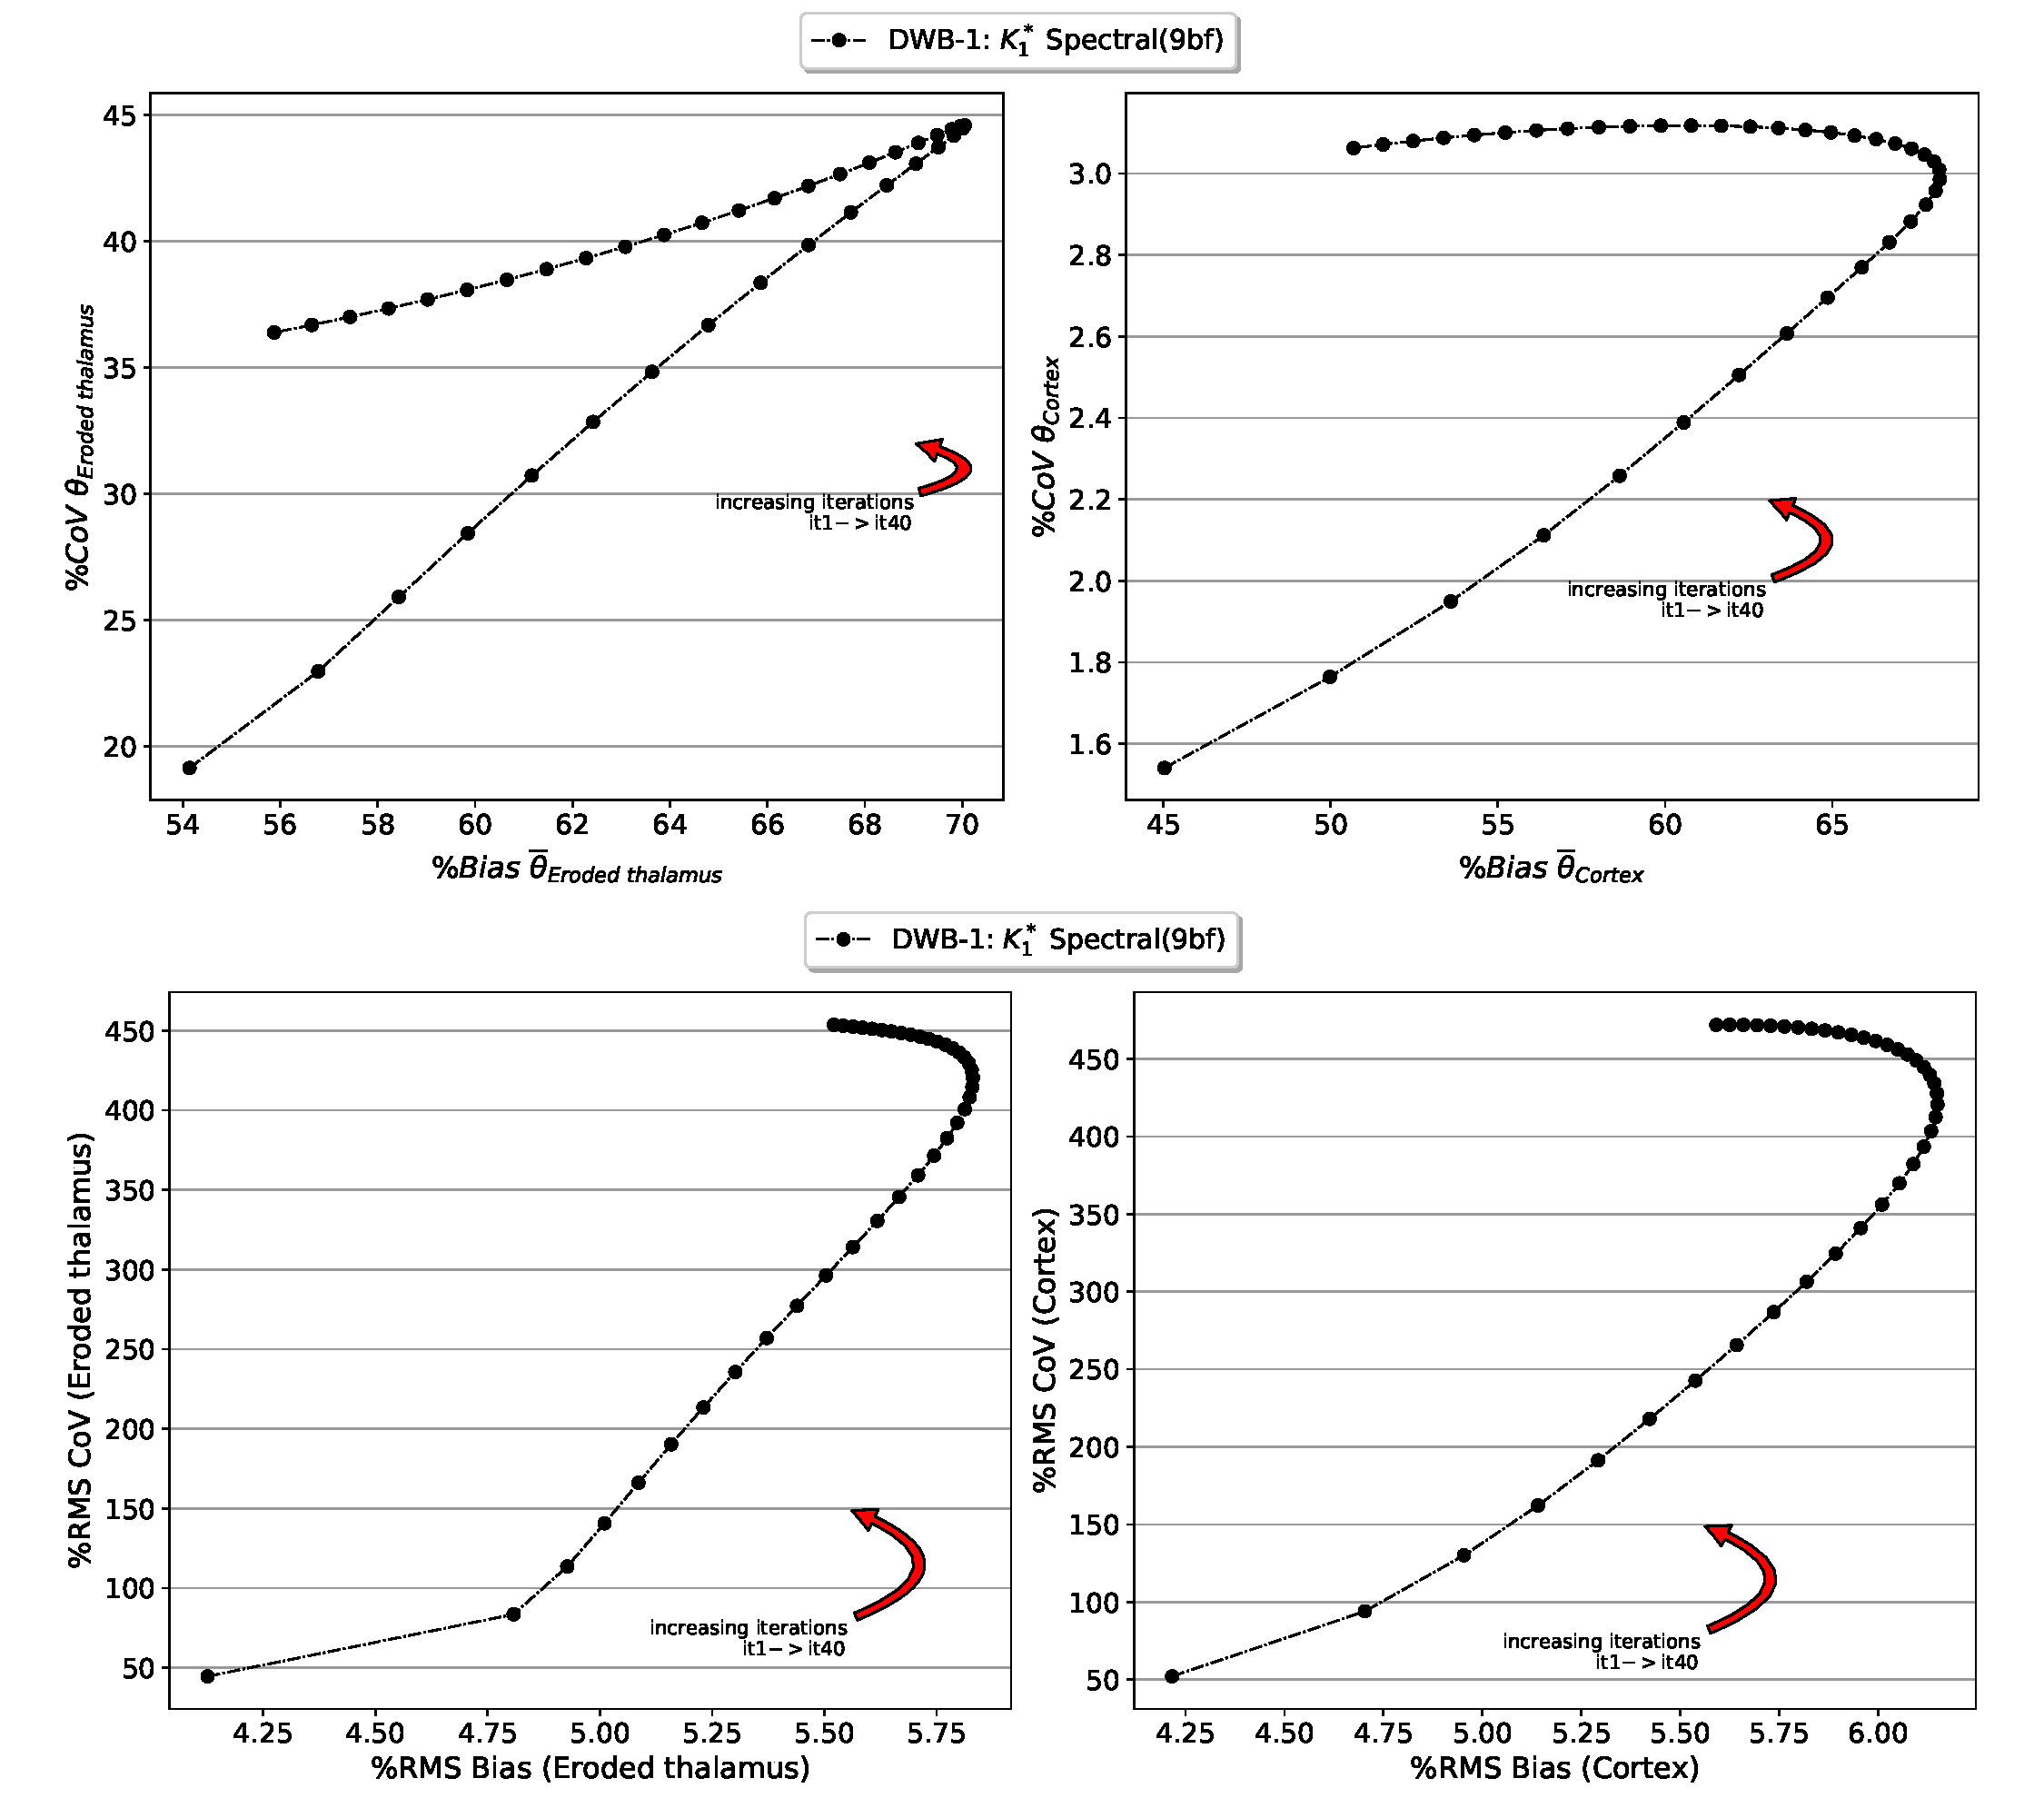
\includegraphics[scale=0.45,angle=0]{3_Results/3_2_Dynamic_Reconstruction_SimulationStudy/figures/VOI/K1_WB1.pdf}
\caption{Simulation: Eroded thalamus (left) and Cortex (right) noise versus bias trade-off curves for $K_1$ parametric imaging from 4D spectral reconstructions of the simulated DWB-1 protocol data. VOI based metrics (top row) and voxel-based metrics (bottom row).} 
\label{fig:K1_WB1}
\end{figure} 

\begin{figure} [ht!]
\centering
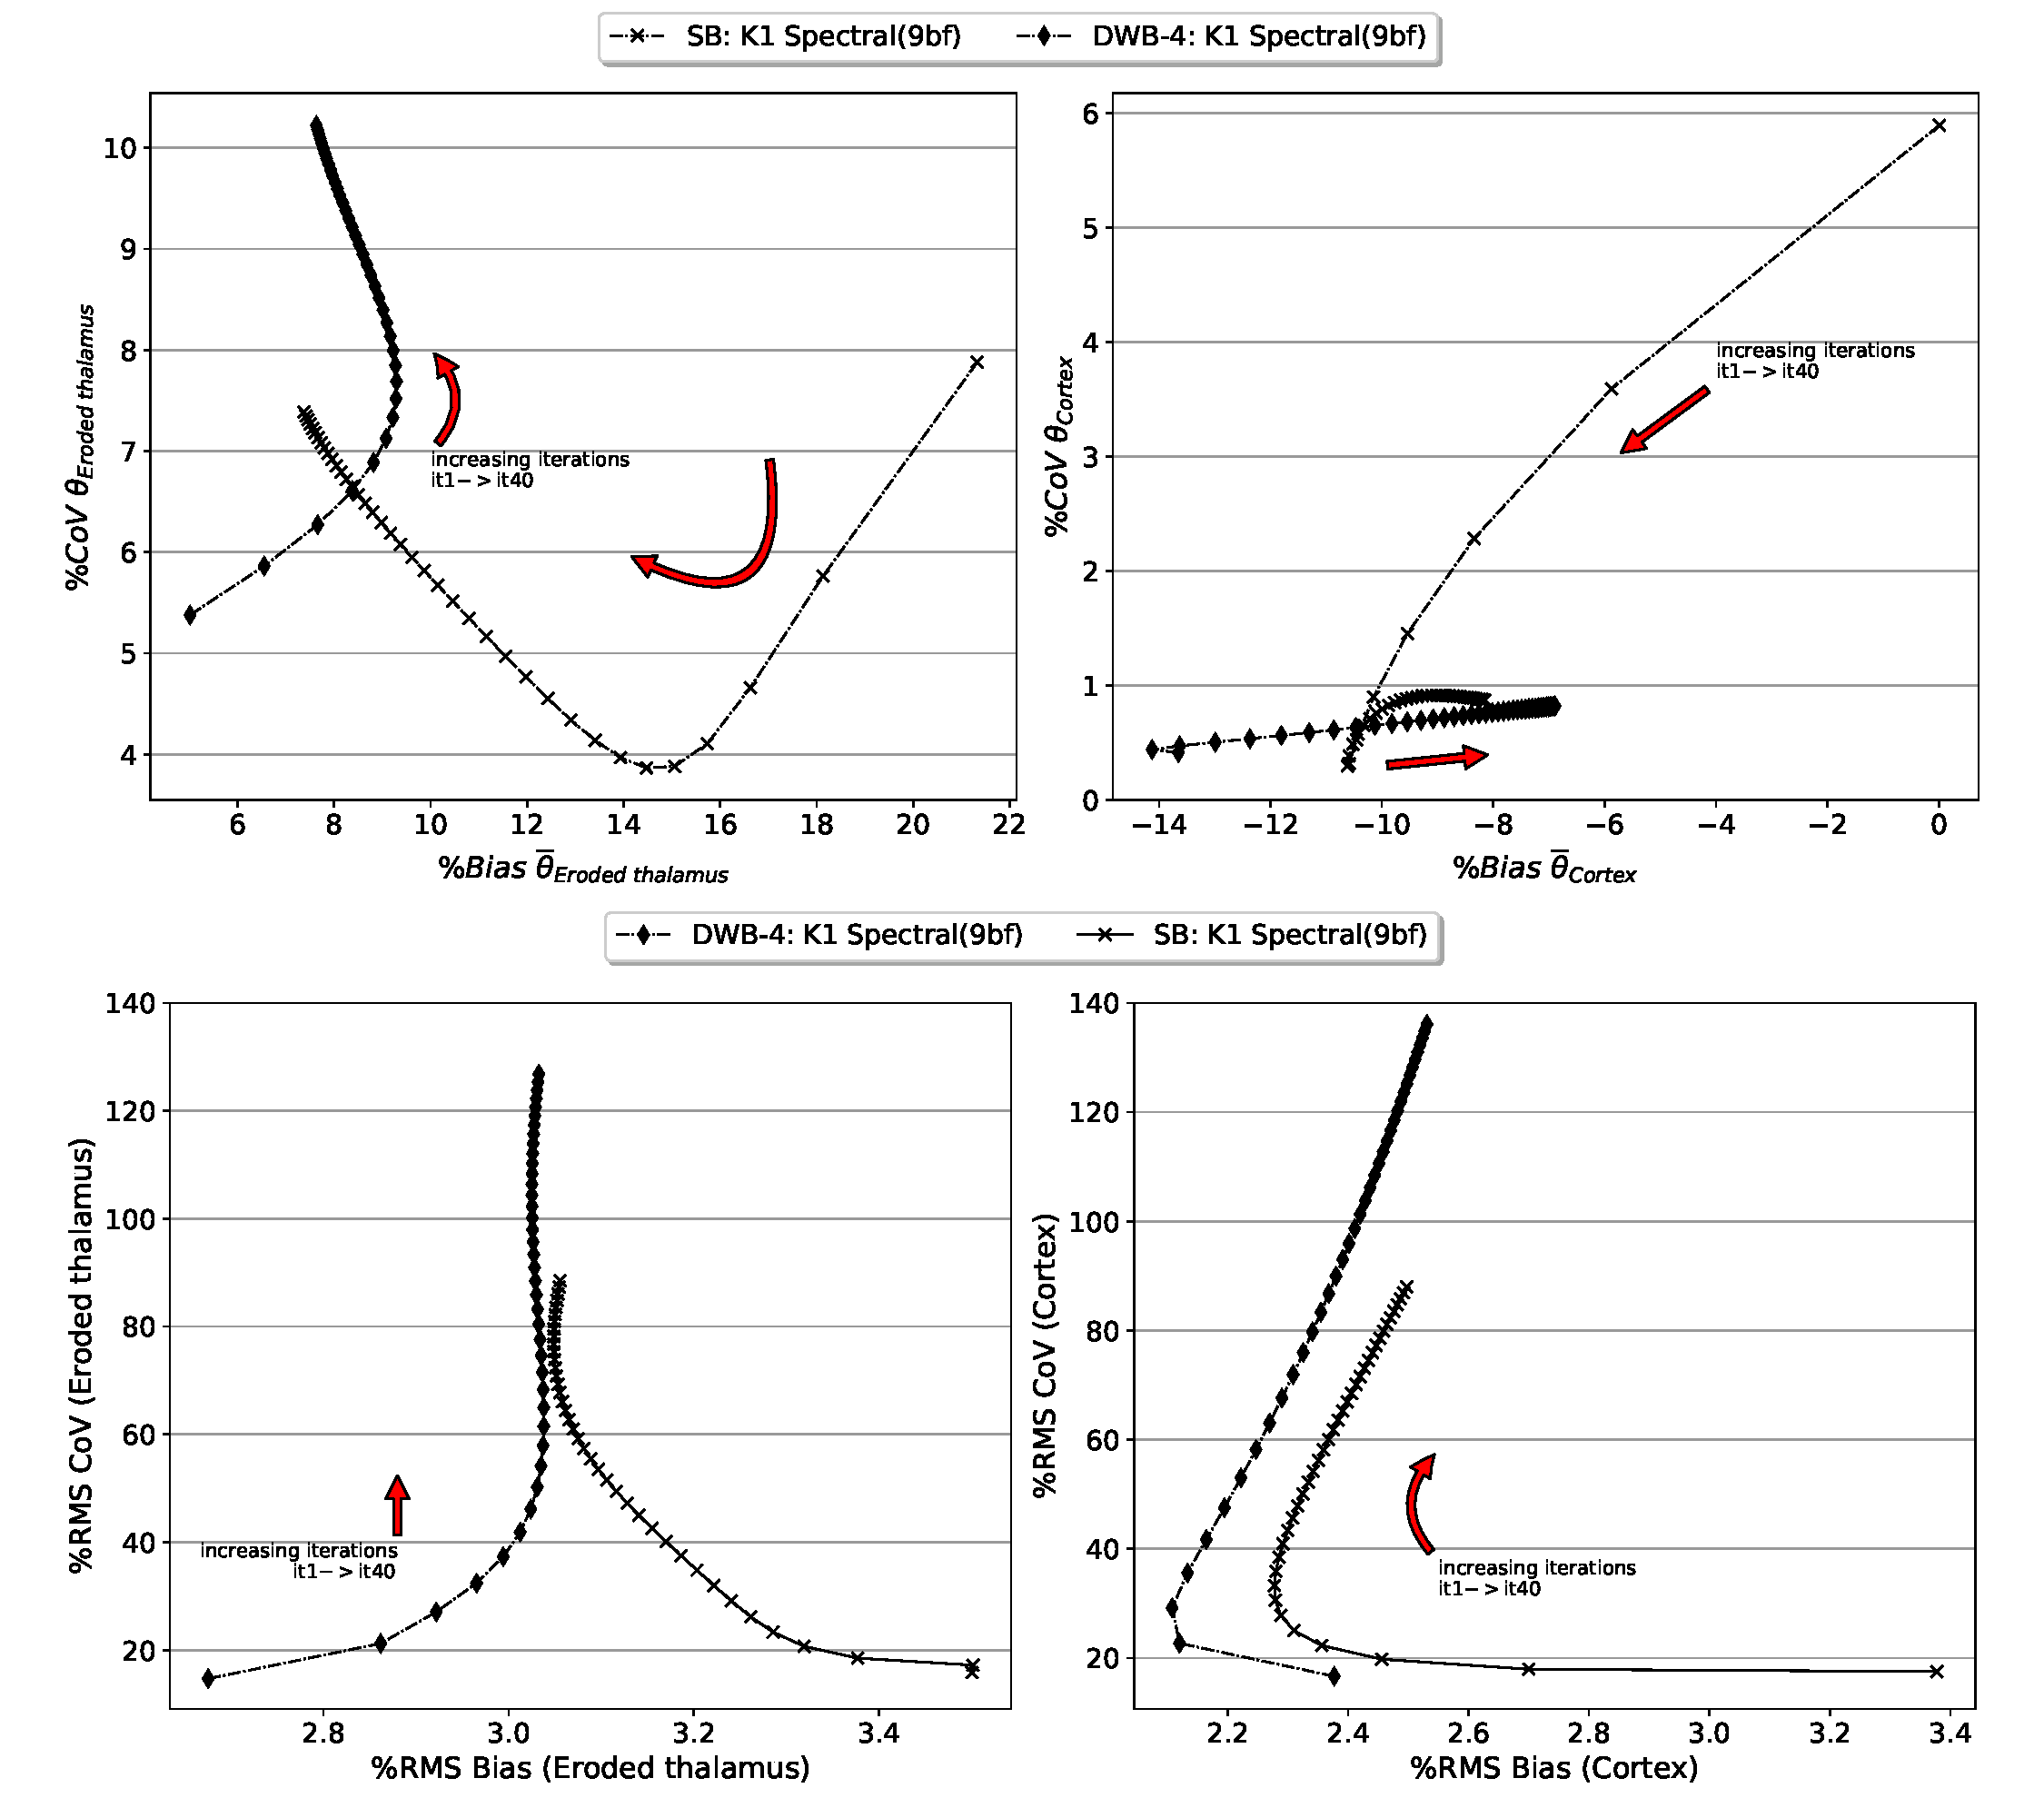
\includegraphics[scale=0.45,angle=0]{3_Results/3_2_Dynamic_Reconstruction_SimulationStudy/figures/VOI/K1_WB4.pdf}
\caption{Simulation: Eroded thalamus (left) and Cortex (right) noise versus bias trade-off curves for $K_1$ parametric imaging from 4D spectral reconstructions of the simulated SB and DWB-4 protocol data. VOI based metrics (top row) and voxel-based metrics (bottom row).} 
\label{fig:K1_SB_WB4}
\end{figure} 

\begin{figure} [h!]
\centering
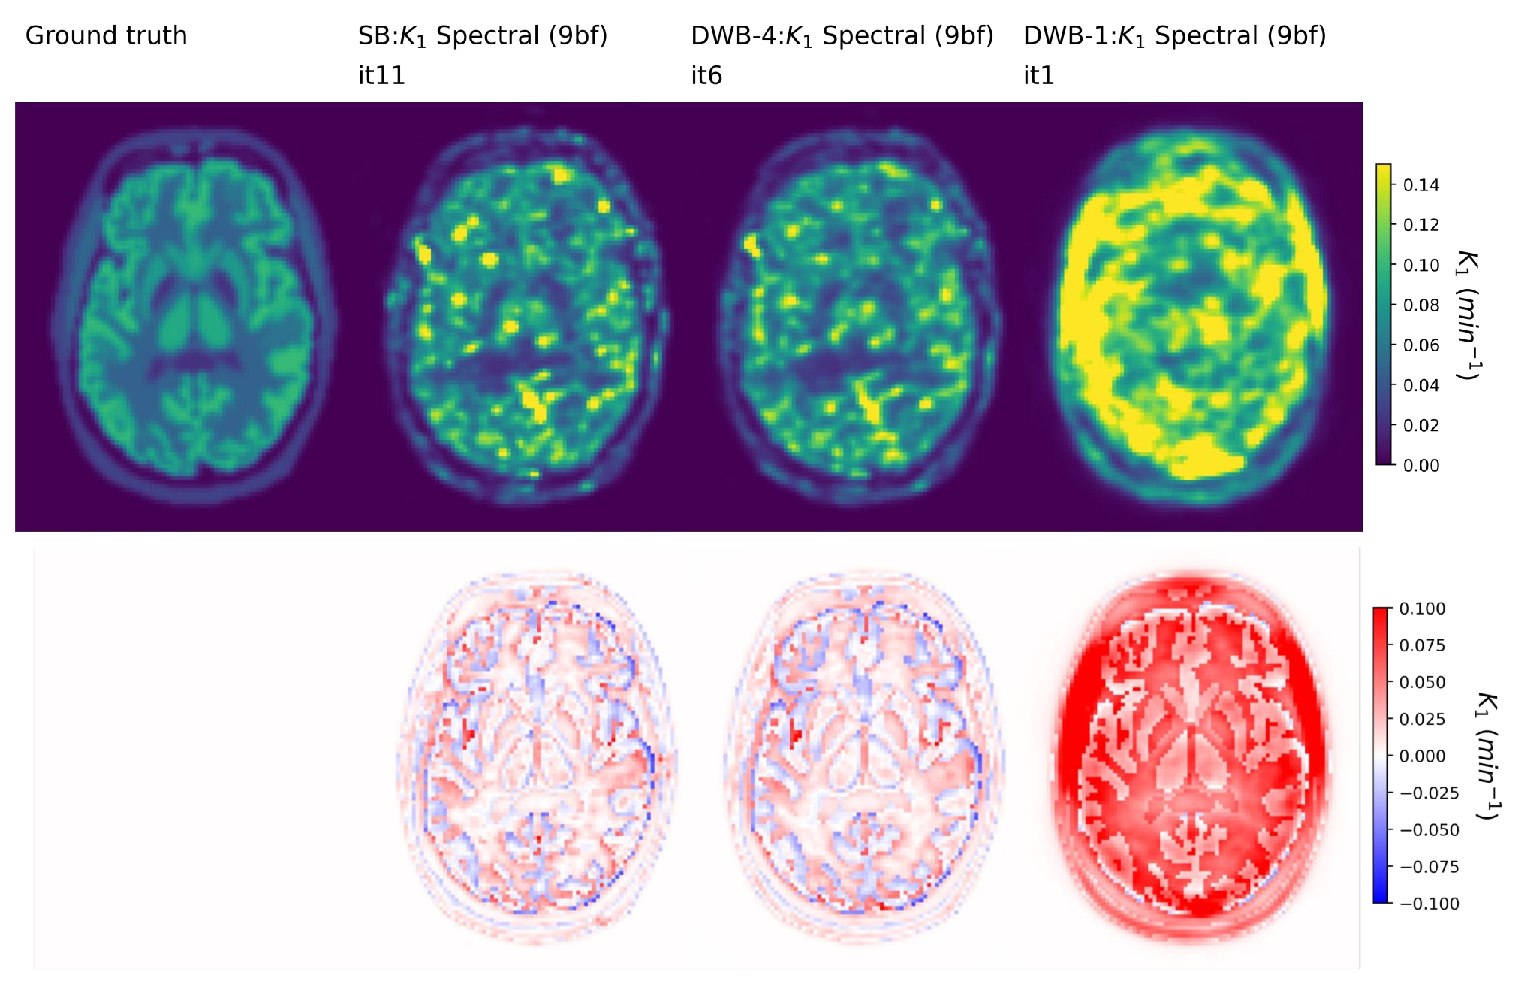
\includegraphics[scale=0.47,angle=0]{3_Results/3_2_Dynamic_Reconstruction_SimulationStudy/figures/BrainCuts/K1_BrainCuts.pdf}
\caption{Single slice though parametric $K_1^*$ images of one noise replicate (with 3mm Gaussian Filtering) (top) and their corresponding Bias images (over noise replicates) (bottom) from SB and DWB data 3D and 4D reconstructions at matched RMS CoV in the eroded thalamus.}
\label{fig:K1_cuts_bias_matched_rms_CoV}
\end{figure} 


\section*{Discussion}
Our simulation study shows that the dynamic reconstruction of DWB FDG data resulted in substantial reduction of Patlak $K_i$ image noise and more favourable convergence behaviour, compared to 3D reconstruction based parametric imaging. These results, limited to a single level of noise, are in agreement with the findings of~\cite{Karakatsanis2016a}. 
Moreover, we directly compared against a SB dynamic protocol, processed with 3D reconstruction, and showed that comparable values of parametric image noise and bias can be achieved with DWB protocols by the use of a dynamic reconstruction.
% Choice of iteration 
The choice of the iteration number to terminate a 4D reconstruction algorithm is not evident.
For a VOI-based analysis, the convergence of the mean $K_i$ value in the cortex or in the eroded thalamus was not seen in the range of the 40 evaluated OSEM iterations, in particular for a 3D reconstruction. This behaviour was also observed for a 4D reconstruction algorithm, but to a lesser extend. A high number of iterations of 4D reconstruction algorithms provided more stable VOI mean values, but at risk of resulting to higher parametric image noise than that of a 3D reconstructions on the same DWB data. 
%Furthermore, parametric image characteristics on each iteration will depend on the underlying data noise, the number of frames and other factors that will be application and potentially exam specific.
The results obtained with one real data-set showed similar behaviour with mean VOI values continuing to slightly increase even after 40 OSEM iterations and with 4D reconstruction parametric image noise surpassing that of 3D reconstruction at late iterations.
This example illustrates that the relative aspects of 4D to 3D comparisons with simulated data for the tested DWB and SB protocols have the capacity to translate to studies with different levels of noise. %A limitation in this comparison with real data is that the use of TOF in real data can alter the convergence behaviour which could potentially explain the differences seen in the evolution of CNR with iteration. Nonetheless, the ranking of the reconstructions with respect to the result CNR was similar between simulation and the real study.
%A limitation in the comparison against the real study was the use of TOF reconstruction, potentially also with the use of TOF reconstruction which was the case in the real data example but not in our simulation study. 
Overall, the risks of excessive parametric image noise and under-converged $K_i$ values will be lesser for 4D based reconstruction methods than for a 3D reconstruction, which demonstrated considerably more instability with increasing iterations. To ensure convergence of the $K_i$ values while suppressing the increase of parametric image noise, further regularisation techniques can be used with methods such as 4D MAP reconstruction~\cite{Reader2014,Wang2008} or kernel 4D dynamic reconstruction~\cite{Novosad2016b,Gong2018}.

% NNLS optimization
Our nested optimization tests using NNLS instead of multiple MLEM sub-iterations did not provide any differences in the acceleration of the convergence and showed comparable behaviour to a previous study on the use of NNLS with the spectral model~\cite{Matthews2010}. 
NNLS did provide computing acceleration by a factor of around two for our data sets, but resulted in an increase of the parametric image noise compared to MLEM sub-iterations for similar bias characteristics.
Equivalent or higher acceleration could be potentially achieved if the nested MLEM optimization was conducted in graphical processing units (GPU) instead of the CPUs.

% Use of the Spectral reconstruction - benefits 
In this work, we evaluated the use of an indirect dynamic reconstruction method based on a generic 4D Spectral reconstruction algorithm followed by a post-reconstruction Patlak model fitting. 
The genericity of the spectral model allows for flexibility in modeling dynamic processes that do not necessarily fall under the idealised behaviour of the kinetic model of interest.
In this simulation study, we were limited to irreversible FDG kinetics that can be sufficiently described by the Patlak model. 
In this case, 4D Spectral reconstruction making use of the full dynamic data outperformed the direct Patlak reconstruction in terms of parametric image noise, while maintaining similar bias behaviour. 
The benefit of the 4D spectral reconstruction was less obvious when fewer frames were used in reconstructions using $t>t_{ss}$, indicating that its favourable behaviour was mostly due to the use of more temporal frames than the Patlak reconstruction.
In real FDG studies, it can be desirable to account for reversible FDG kinetics and reduce the bias of the estimated macro-parameters arising from poorly modelled kinetics. 
The spectral model can allow for more complex compartmental modeling with no strong prior knowledge or enforcement of a specific model. 
As such it can account for more complex kinetic behaviours, including reversibility of tracer, in the reconstruction process 
and allow for post-reconstruction exploratory modeling to identify the best model to describe and present the data. 
Moreover for DWB studies where not all body regions and organs will necessarily be adequately described by a single dynamic model of interest, 
the proposed indirect method can allow for the assignment of different kinetic models in different regions of the body to ensure appropriate representation of the dynamic tracer behaviour.
Depending on the availability of early frame data, the fitted spectral model can be used to directly estimate $K_1$~\cite{Meikle1998,Matthews2010}, 
while post-reconstruction micro-parameter estimation could be performed for potential uses in clinical applications~\cite{Novosad2016b,Zaker2020} and indirectly take advantage of the 4D reconstruction temporal regularisation.
% Number of basis functions
An important parameter to configure for the spectral model is the number of basis function. 
Contrary to post-reconstruction spectral analysis where hundreds of basis functions are used to finely sample the space of kinetic exchange rates, a smaller number of basis is desirable in reconstruction to favour reduced image noise.
In some cases of our findings the lowest number of basis functions used (6 basis) resulted in higher bias values which indicates less than adequate modeling of the underlying kinetics, compared to reconstructions with more basis functions and to 4D Patlak reconstruction. However this was not the case when fewer frames were used in reconstructions using $t>t_{ss}$ data. 
These findings indicate that the selection of number of basis functions is important not only for controlling the produced image noise but also for controlling bias by adequately modeling the kinetics behaviour in reconstruction. 
For the higher numbers of basis functions, with 9 and 17, almost identical behaviour was seen on the DWB-1 dataset (of 8 frames). 
Overall on the choice of number of basis functions, results indicate a greater risk in image bias when using a too small number of basis functions, and a lesser risk in image noise when using more basis functions than strictly needed to properly model the underlying kinetics.
In any case the number of basis needs to be tuned for every DWB protocol, depending on the number of frames within the dataset and the range of underlying kinetics as well as the level of noise in the PET data.

% DWB Protocols comparison
In this study, the investigation between S\&S and CBM DWB protocols was limited to aspects of sampling frequency and uniformity within the total examination time. 
Our results showed small differences in parametric image bias but noticeable reduction in parametric image noise when utilising CBM acquisition with uniform sampling. 
Overall differences were inline with previous findings of comparison S\&S and CBM on a real data study using different metrics~\cite{Karakatsanis2016b}. 
A limitation in our study is that we have considered a single axial location and hence we cannot generalise the results of the simulation study for the performance of the assumed DWB protocols over their effective FOV. 
Furthermore beyond the aspects of reduced acquisition delays and higher sampling frequency, CBM acquisition has other desirable properties for DWB acquisitions as outlined previously~\cite{Karakatsanis2016b}. 
The most important aspect is the result uniform axial sensitivity profile at any choice of acquisition speed. 
That can be of importance in DWB parametric imaging where multiple regions of interest are expected in the effective FOV.
In our study we have not considered this aspect for the CBM protocols and we did not examine regions in the overlap range of the S\&S protocol. 
But the observed improvements related to reduced delays in acquisition coupled with uniformity of axial sensitivity favour the choice of CBM over S\&S protocols. 
We investigated further potential reductions in system delays by allowing for non-uniform axial sampling using bi-directional CBM.
In that case we did not see the same effects as in the transition from S\&S to CBM. % , which can potentially be attributed to the non-uniform sampling nature of bi-directional protocols.
But our results on bi-directional CBM are limited to the specific framing of the evaluated protocol design which offered more total frames but resulted in less total counts compared to the other protocols. Additional tests are required on the exploitation of the flexibility offered by bi-directional CBM to assess other potential benefits against uni-directional CBM.

\textcolor{blue}{
Finally an additional evaluation was made for parametric $K_1$ imaging, by use of the spectral model and the spectral coefficient images, to explore additional potential benefits from the use of 4D Spectral reconstruction in parametric imaging. The tests showed, as expected from previous single bed dynamic studies~\cite{Meikle1998}, that the first few minutes of the acquisition are crucial for the estimation of $K_1$. Estimates of $K_1$ were erroneously biased and noisy for estimates that made only use of late dynamic data, as shown with $K_1$ imaging from DWB-1 protocol data. The DWB-4 protocol that made use of the first 3 minute acquisition provided results that were very similar to those of the single bed protocol data with no gaps. These results are promising for the estimation of $K_1$ parametric images from DWB protocols that include an initial single dynamic bed phase, which is off course limited to the areas covered by this initial acquisition.
A considerable limitation in our tests for $K_1$ parametric imaging using 4D Spectral reconstructions is that quantification accuracy was compromised by not considering the blood volume fraction in $K_1^*$ estimation. This was done to avoid excessive parametric image noise by the division operation that is required by equation~\ref{eqn:SpectralCPET_AllEquations} to correct $K_1^*$ for blood volume fraction. 
Alternatively to completely neglecting the blood volume fraction correction, a constant value could be assumed for certain regions of the image or smoothing and other denoising operations could be performed on the 4D spectral reconstruction estimated blood fraction image $\phi_M$ before being applied to the $K_1^*$ image via division.}

\section*{Conclusion}
4D dynamic reconstruction is necessary in DWB parametric imaging to achieve accurate and stable quantification. For FDG Patlak $K_i$ parametric imaging we have shown results of direct Patlak dynamic reconstruction with noise and bias values that were comparable to 3D reconstruction based parametric imaging from single bed dynamic studies. 
In this work we proposed the use of an indirect method for DWB parametric imaging, based on the spectral analysis model. This more flexible approach allows for complex kinetic modelling to be used during reconstruction for temporal regularisation, with minimal assumptions on the underlying kinetics. In Patlak $K_i$ parametric imaging this method outperformed the direct Patlak approach, by making use of all the acquired data for temporal regularisation from which post-reconstruction parametric imaging benefitted by further reduction of noise compared to the Patlak approach. Furthermore, the spectral model approach can be used for more complex post-reconstruction modelling, for example in parametric imaging of FDG micro-parameters.
\textcolor{blue}{In our evaluation we showed that in addition to post-reconstruction fitting, dynamic reconstruction with the spectral model can be used for estimation of $K_1$ parametric images when early dynamic information are available.}

Finally, we investigated the impact of various acquisition modes (for CBM and S\&S) resulting in different temporal sampling of the data. Benefits of reduced delays and increased acquisition statistics were partially seen in reduced parametric image noise for the CBM protocol with uni-directional axial sampling. By contrast CBM using bi-directional motion resulted to parametric image noise levels that were similar to the S\&S protocol. Further investigation is required to assess the potential benefits from bi-directional CBM against uni-directional CBM and effects of non-uniform sampling over the entire FOV of the DWB protocols.

Overall, use of 4D dynamic reconstruction for DWB parametric imaging offers desirable properties that enables the transition from single bed dynamic studies and common 3D reconstruction parametric imaging practices without loss of image quality and with additional benefits for accuracy of parametric images. 
Potential applications of DWB parametric imaging are expected to rely on quantification of images and so there should be no compromise between parametric image accuracy and image noise. Our results showed that 4D reconstruction need to be sufficiently iterated to ensure accurate quantification, with potential for improvement in maintaining low parametric image noise by use of additional regularisation methods.



\section{Conclusions to this Chapter}
Dynamic reconstruction capabilities were successfully developed and validated in CASToR, for multiple dynamic models and optimization algorithms. Along with dynamic developments for a PET analytical simulator, those tools have enabled an extensive evaluation of dynamic reconstruction methods for application in DWB imaging. The developed tools were used for the application of dynamic reconstruction on real data and were further evaluated and expanded, in the work that is described in the following chapter, for real DWB data.